%%%%%%%%%%%%% You can ignore this stuff
\documentclass[bsc]{abdnthesis}
\usepackage[T1]{fontenc}
\usepackage[utf8]{inputenc}
\usepackage{booktabs}
\usepackage{longtable}
\usepackage{csquotes}
\usepackage{minted}[linenos, breaklines]
\usepackage{url}
\usepackage{pdflscape}
\usepackage{tikz}
\usepackage{pdfpages}

\usepackage[style=apa, backend=biber]{biblatex}
\DefineBibliographyStrings{english}{%
  bibliography = {References},
}
\addbibresource{library.bib}

% This creates hyperlinks and moves the contents links to the page number for clarity
\usepackage[linktocpage=true,hidelinks]{hyperref}	

\def\subsectionautorefname{Section}
\def\subsubsectionautorefname{Section}
\def\sectionautorefname{Section}
\def\chapterautorefname{Chapter}

%%%%%%%%%%%%%%%%% Space for your own packages here %%%%%%%%%%%%%%%%%%%%%%%%%%%%%%
% Uncomment for blank lines between paragraphs rather than
% indents
\usepackage[parfill]{parskip}

%%%%%%%%%%%%%%%%%%%%%%%%%%%%%%%%%%%%%%%%%%%%%%%%%%%%%%%%%%%%%%%%%%%%%%%%%%%%%%%%%

\title{Using AI to Predict Bangladesh's Drinking Problem}
\author{Kane Swartz}
\upnumber{941226}

\projecttype{Research Project}
\school{School of Computing}

%%%% In the final submission of a thesis, this should only be the year
%%%% of submission.  However, it is useful to use \date{\today} for drafts so that
%%%% they don't get mixed up.
    
\date{2023}

%% It is useful to split the document up as chapters and include
%% them.  LaTeX will sort out all the numbering and cross-referencing
%% for you --- if you run it enough times!

\begin{document}

%%%% Create the title page and standard declaration.

\maketitle
\makedeclaration

%%%% Then the abstract and acknowledgements

\begin{abstract}
  The drinking problem referred to in the title is groundwater arsenic pollution. This project aims to evaluate existing expert system predictive models developed in the University of Portsmouth and compare them to machine learning based models.

  In 2023 machine learning and artificial intelligence are becoming ever more prevalent, this dissertation explores the potential impact this field could have on predicting the arsenic pollution of groundwater.
\end{abstract}

\begin{acknowledgements}
  iArsenic has been foundational to this project. The dataset extracted from iArsenic has been a huge asset and represents hours of high quality work from all of the iArsenic team who have ensured source data has been cleaned and aggregated to a high standard.

  Thank you to Dr Mohammed Hoque, the initial visionary for iArsenic and client to this project. Dr Jacek Kopecký for leading the development of the iArsenic web application and the following contributors in the iArsenic team:
  \begin{itemize}
      \item Dillon O'Shea (TingeOGinge)
      \item Lewis Knewton (lewisknewton)
      \item Nylah Daniella Klasson (TxJson)
      \item Benjamin Kyd (benkyd)
      \item Fionn Plant (CybrChick007)
      \item AloysT
      \item PreslavPO
  \end{itemize}

  Additional thanks to my supervisor Dr Rich Boakes and friend and mentor Dr David Ralph, who have each provided key direction leading up to and throughout the development of this project.
\end{acknowledgements}

%% please indicate whether you are happy for other students to
%% view your project in the future
\section*{Consent to Share}
I consent for this project to be archived by the University Library and potentially used as an example project for future students.

%%%% These are macros ( each macro is defined by \newcommand )
%%%% These macros make cross-referencing easier, building on the
%%%% already very useful \autoref{ref}.  You tweak them or build your own. for \end. !!!
% !!! Environment ended while waiting 
%% \autorefp{ref}
%% Like \autoref, but adds the page number
%% e.g. Section 3.2.4 (p345)
\newcommand{\autorefp}[1]{\autoref{#1} (p\pageref*{#1})}

%% \autorefnp{ref}
%% Like \autoref, but adds both the section name and page number
% e.g. Section 3.2.4 "blah blah" (p345)
\newcommand{\autorefnp}[1]{\autoref{#1} ``\nameref{#1}'', (p\pageref*{#1})}

%% \see{ref}
%% Handy shorthand for inserting a hyperlinked xref.
%%   e.g. (see Section 3.2.4, p134)
%%        (see Figure 5.1, p23)
%%        (see Table 4.7, p999)
\newcommand{\see}[1]{\hyperref[#1]{(see \autoref*{#1}, p\pageref*{#1})}}

%% \seenamed{ref}
%% Handy shorthand for inserting a hyperlinked xref that also includes
%% the name of the section being referred to.
%% (see Section 3.2.4 "blah blah", p134)
%% (see Figure 5.1 "blah blah blah!", p23)
%% (see Table 4.7 "blah blah blah blah blah blah", p999)
\newcommand{\seenamed}[1]{\hyperref[#1]{(see \autoref*{#1} ``\nameref*{#1}'', p.\pageref*{#1})}}

%% \bq Block Quotations.
\newcommand{\bq}[2][]{\singlespacing \begin{quote} 
\begin{small} ``\textit{#2}'' \end{small} #1 \end{quote} \doublespacing}

%% \qq{quotation}for \end. !!!
%%!!! Environment ended while waiting 
%% Shortcut for doing inline quotations (with 6699 quotation marks around italic text)
%% e.g. \qq{To be, or not to be}
\newcommand{\qq}[1]{{\enquote{\textit{#1}}}}

%%%% It should have a table of contents, but delete the other two as
%%%% necessary.

\tableofcontents
\listoftables
\listoffigures

\chapter{Introduction}

\section{Background and Historical Context}

Arsenic pollution in groundwater is a problem faced worldwide \parencite{khan2014groundwater}. Southeast Asian populations, particularly those of Bangladesh, are arguably the most negatively impacted by arsenic contamination in drinking water worldwide. 

 \parencite{Smith2000}. 

These tube wells were typically installed at a depth of under 200 meters. Arsenic concentrations in groundwater peak at between 15 and 25 meters of depth and are typically only below the World Health Organisation's safe arsenic limit of 10$\mu$g/litre \parencite{WHO2003} at 200 meters of depth or more \parencite{Chakraborti2010}. 

Prior to the discovery of harmful levels of arsenic in the water from these tube wells, their installation was acclaimed as a huge success with regards to providing the population with clean drinking water \parencite{khan2014groundwater}. Tubewells today are still extremely popular in Bangladesh with approximately 95\% of rural people and 70\% of urban people using them in 2020 \parencite{Ghosh2020}.

\subsection{Solution Approach}

\cite{Smith2000} emphasizes that the core of any solution must be to provide non-polluted water.

This article makes it clear that there is no single solution to this issue, it may seem simple to provide water filters, for example, but for their successful deployment, they must be provided with education and community engagement to ensure their efficacy. They are also not a permanent solution. 

\cite{Khan2014} illustrates the scale and complexity of a comprehensive solution approach by analysing the motivations of key stakeholders.

\section{What is iArsenic}

iArsenic is a web application that estimates the arsenic concentration for a well in Bangladesh based on its geographic region, depth and visible staining on the well.

This is achieved by aggregating source data about these wells and using that aggregate data to produce expert system prediction models which are available via a web application.

The tooling developed to produce these models are general purpose and modular, enabling them to be imported into other projects. The time and expertise required to clean and aggregate the source data used by these models are very substantial and leveraging this existing work allows higher level outcomes to be brought into scope.

The data in iArsenic has been selected from reputable sources and represents a large and high quality dataset, representing the majority of Bangladesh.

\section{Research Questions}
\label{RQ}

1. What is the performance of the existing iArsenic models.

2. Do machine learning models have potential in the prediction of groundwater arsenic pollution?

\section{Conclusion}

Arsenic pollution is a serious and ongoing issue and it is a great shame that despite relevant organisations being aware of this problem since at least the year 2000 it persists to today in 2023.

This project does not aim to conquer and eliminate this problem, but does aim to make a contribution to the ongoing research into the use of predictive models to predict groundwater arsenic pollution.

To achieve this contribution, this project aims to validate existing predictive models and provide an example for the application of machine learning in this field.
\chapter{Literature Review}

This chapter outlines the existing systems being used to predict the safety of drinking water sources in Bangladesh and other regions where applicable, the tooling and techniques required to implement and evaluate new prediction models and touches on the considerations and limitations of these models with regard to the black box problem. 

\section{Existing Work}
\label{ew}

\subsection{iArsenic}

The existing iArsenic models are expert system models. This type of model follows rules defined by an expert in the field, this can be thought of as a flow chart. This approach has the benefit of the output of the model being explainable and justifiable; a white box model. 

Expert systems can be limited compared to machine learning-based models as the decision boundaries made by an expert system are defined by an expert, whereas machine learning algorithms will statistically identify decision boundaries.

In total there are 5 iArsenic models, each has been developed sequentially, improving on the one before. Initially written in R, 3 of the iArsenic models, model3, model4 and model5, have been converted to NodeJS / JavaScript and uploaded to GitHub.

The iArsenic models are documented at this link: \url{https://github.com/portsoc/iArsenic/tree/master/preprocessing}

\subsection{Predicting Arsenic Concentrations with Surface Parameters}

\cite{Winkel2008} page 536 used latitude, longitude and surface parameters from the Food and Agriculture Organization of the United Nations to predict arsenic concentration in groundwater. This was done by calculating the correlation coefficient between these surface parameters and arsenic concentrations for use as global parameters in a classification model. This model achieved a true positive and true negative rate of 65\% over multiple countries in Southeast Asia.

\subsection{Satellite Mapping of Flooding Patterns}

\cite{Connolly2022} page 928 uses high-resolution satellite data combined with surface parameters to predict groundwater arsenic concentrations within an area of 30m using a random forest model. The results in this article are not comprehensive, though a figure for a sensitivity rate of 95\% for wells with arsenic concentrations of over 10µg/l is provided.

The compromise for this high sensitivity level appears to be that the dataset covers a smaller area than the iArsenic dataset, which covers the majority of Bangladesh or \cite{Winkel2008}'s dataset which covers several countries in Southeast Asia.

\textbf{Conclusion}

While \cite{Connolly2022}'s model achieving a sensitivity rate of 95\% is the highest for any model found in this literature review, this does not provide a comprehensive performance evaluation for the model. A model which always predicts true will have a sensitivity of 1.

\cite{Winkel2008}'s model provides a more robust evaluation by providing a receiver operator curve.

It is not possible to generate a receiver operator curve for the iArsenic models. This is because the models do not provide a feature to change the classification threshold. It is possible to generate the f1 score, sensitivity and specificity. This will factor in the true positive rate and true negative rate. See these terms defined at \ref{EM} on page \pageref{EM}.

\section{The Black Box Problem}

\cite{Fleming2021} states that acceptance of machine learning-based approaches have faced resistance in earth \& environmental sciences due to the inability to explain how machine learning models are working and the lack of understanding of artificial intelligence in the earth \& environmental field. While this is partially true in terms of the black box problem there is are examples of machine learning being used to analyze groundwater quality. A more difficult question to answer is whether these models are less applicable in real life compared to human-designed models, as is asserted by \cite{Guidotti2018}.

In machine learning, the black box problem is based on the inability to explain how a model produces an output for a given input.

\cite{Castelvecchi2016} illustrates this issue with the following, imagine a black box machine learning model was created with a set of images of mammograms including labels indicating whether the person in the scan went on to develop breast cancer. It could happen that this model outperforms human medical professionals in predicting whether someone would go on to develop breast cancer.

One could argue that the benefit of this model would be that it could identify when women should have a preventative mastectomy. However, critics assert that critical decisions cannot be made without justification and that one cannot justify a decision that cannot be explained (\cite{Loyola-Gonzalez2019}). The human doctor's opinion will always be explainable, by the doctor themselves.

Not all machine learning base models are considered to be black box systems. Decision tree models for example are powerful machine learning tools which produce models considered white box systems meaning you can analyse them to determine how they're working \parencite{Caruana2006}. Decision tree models can be contrasted with neural network style models which are almost always considered black box models.

Because determining whether a drinking water source is safe does factor into critical decision-making, it is important to explore the black box problem. The purpose of this project, however, is to compare the performance of a predictive model developed with machine learning to existing expert system models. Therefore whether a model is black or white box will not be a critical factor in model selection.

\section{Tool Selection}

\subsection{Model Implementation}

Preliminary investigations into machine learning, including speaking to local experts at the University of Portsmouth, identified three potential systems for designing and implementing machine learning frameworks, scikit-learn, WEKA and TensorFlow.

\textbf{scikit-learn}

Scikit-learn provides a well defined Python interface for a wide range of well defined machine learning models and techniques. This makes scikit-learn good for implementing existing model architecture but limits the development of new architectures. This makes scikit-learn less suitable for custom architectures and deep learning than tools such as TensorFlow. 

Its Python interface does mean however that it does not limit the possibilities of preprocessing or post-processing the input and output of a model (\cite{scikit-learn2023}).

\textbf{TensorFlow}

TensorFlow contrasts with scikit-learn by allowing full access to the model architecture. This makes it suitable for both deep learning and supervised learning. TensorFlow can also follow a distributed architecture, allowing it to scale to larger datasets. This versatility however greatly increases the complexity of the tool in comparison to WEKA or scikit-learn (\cite{Google2023}).

TensorFlow provides GPU support, which could be used to decrease the time taken when testing and training, allowing less optimization to be applied to models.

\textbf{WEKA}

Of the three tools for model implementation considered, WEKA is the most simple to use, providing a graphical user interface. While this simplicity means WEKA is very easy to use, it is also limited in its versatility, providing a limited API, making it difficult to integrate with the iArsenic models and fewer model types and configuration options compared to scikit-learn or TensorFlow (\cite{Waikato2023}).

\textbf{Conclusion}

Scikit-learn has been chosen to develop and run the models because of its standardised Python based model interface. WEKA was not deemed suitable because it provides no easy way to integrate with Python or NodeJS. TensorFlow would be a suitable choice but is less appropriate than scikit-learn due to the complexity it introduces.

\subsection{Python Dependency Management}

This section will outline and compare the potential choices for dependency management.

Good dependency management allows a Python project to be added to a different machine and for that project's dependencies to be installed without clashing with the existing Python dependencies of that system. Without this, the code can become tied to the developer's system-wide Python installation and prevent other Python projects from being unable to run, where they require different versions of the same package as another Python project on the system.

\textbf{Conda}

Conda is a high-level environment and package dependency manager which works with Python and other languages. The appeal of Conda is the simplicity of the user experience. Conda manages every aspect of environment and dependency management. This, however, comes at the cost of the complexity of the tool itself. Portability and collaboration is a concern with Conda, as to run it on a virtual machine or another developer's machine, this machine will also need Conda to be installed, which may clash with existing dependency management solutions (\cite{Conda2023}).

\textbf{Virtualenv}

With virtualenv, isolated Python environments can be created and stored in a directory of the project (\cite{virtualenv2023}).

Used in conjunction with the Python package manager, pip, dependencies can be installed to this isolated environment and their version tracked using the pip freeze command. The output of the pip freeze command is conventionally stored in a file named requirements.txt. The requirements.txt file can then be included with the source code and used to install the specific dependencies required for a project.

\textbf{pipenv}

The aim of pipenv is to integrate virtualenv and pip, making it a higher-level alternative to using virtualenv with pip. Practically, the benefit of pipenv is the use of a package.lock file, which allows dependencies to be locked to a specific version, providing a security benefit. This feature however does add complexity and maintainability requirements (\cite{Reitz2023}).

\textbf{Conclusion}

Ultimately virtualenv was chosen for this project due to it being the most simple and lightweight solution, reducing the number of potential failure points when porting to other systems or coming back to this project in the future.

\section{Model Type}
\label{mt}

The initial steps in model selection are rudimentary. Machine learning algorithms can be categorised as, supervised learning, semisupervised learning, unsupervised learning and reinforcement learning. Because our data set consists of structured and labelled data the appropriate choice is supervised learning, see \cite{Aurélien2017} page 24.

Predictions by the existing iArsenic models classify data points as safe, polluted or highlyPolluted. Models produced in this project therefore must produce a comparable output. Predictions from a regression model will not be as comparable to predictions from an iArsenic model as a regression model will output a continuous value. While this would produce valid predictions, it would not be applicable in this project because this estimate will have to be converted to a classification. Therefore the models considered for this project are classification based.

% TODO expand on how these models work

Rich Caruana and Alexandru Niculescu-Mizil provide a comparison of a number of supervised learning algorithms on a range of data sets and performance measures (\cite{Caruana2006}). Based on Caruana's paper and \cite{Aurélien2017} chapter 3, the following model types have been shortlisted for their good performance across a diverse range of dataset types:
\begin{itemize}
    \item k-nearest neighbors classifier
    \item random forest classifier
    \item multilayer perceptron feed forward neural network classifier
\end{itemize}

\subsection{Validating Models \& Minimizing Dataset Bias}
\label{eval}

Bias is always a factor in datasets, some types of bias cannot be measured or controlled, such as sampling bias focusing on collecting data points in and around a city's capital with less focus on rural regions. This may be the case in the dataset used in this project, but further scrutinizing bias is outside the scope of this project. 

The impact of ordering and sampling bias can be minimized however, this section will explore the ways this can be done.

\textbf{Hold Out Validation}

In hold-out validation, the dataset is split into two, a test set and a train set. The train set is used to train a model, then the model is presented with new data to make predictions for. 

This proves the model can generalize to new data, validating its performance. This method is susceptible to ordering and sample bias, however, if for example the dataset is ordered alphabetically.

\textbf{K-folds Cross Validation}

K-folds cross-validation involves splitting the dataset into "k" splits, where k is the number of splits. Each split is then used in turn to be the test dataset and the remaining splits are used for training. Where k equals 5, a model will be trained and tested 5 times. The difference in performance can then be examined between the splits to measure the impact of selection bias (\cite{Aurélien2017} page 99).

\textbf{Shuffle Split Validation}

Shuffle Split validation eliminates ordering bias by randomly selecting a portion of the dataset to be used as the test split. This does however introduce random bias.

\textbf{Leave One Out Validation}

In leave one out validation is similar to k-folds cross-validation, but the number of folds is set to the number of data points. The result is that the model is trained once for each data point and the left out datapoint is used for the model to generate a prediction. Whether this prediction is correct or incorrect for each data point can be used to validate the performance of the model.

This method is good for models with limited data as it minimises statistical power lost by not training the model on the data in the test set. Because it requires the model to be trained and evaluated for every data point, however, it becomes less feasible for models with larger datasets and longer training and evaluation times.

\textbf{Conclusion}

A hybrid of shuffle split k-folds cross-validation has been used in this project. The dataset is first shuffled to eliminate ordering bias then k-folds cross-validation is used to split the data into 5 subsets, allowing us to measure sampling bias.

Leave one out validation is not viable for this project as the dataset contains over 800,000 data points. For the iArsenic model in production, model5, one model instance is approximately 11 megabytes and takes approximately 15 minutes to generate. Therefore this method would take approximately 23 years and require 8.8 terabytes to generate and store the models.

The code to generate the k-folds shuffled split data can be found at \url{https://github.com/JavaRip/UoP-SoftEng-Dissertation/blob/main/utils/src_to_test_train.py#L40-L53}.

\subsection{Evaluation Methods}
\label{EM}

The evaluation method must be applicable to the new models and the existing iArsenic models because the iArsenic models are classification models this section will outline potential classification evaluation metrics and their strengths and weaknesses.

\textbf{Accuracy / Misclassification Rate}

The accuracy of a classification model measures how often the model predicts correctly, usually as a percentage. The misclassification rate is the inverse of the accuracy.

Accuracy as an evaluation metric has disadvantages. If a dataset has an 80\% positive rate, a model which always predicts true will have an 80\% accuracy.

Accuracy: (\(\frac{true\_positives + true\_negatives}{total\_predictions}\))

\textbf{Specificity}

The specificity measures the percentage of correctly classified negative data points; the true negative rate (\cite{Aurélien2017} page 127).

Specificity: (\(\frac{true\_negative}{true\_negative + false\_positive}\))

\textbf{Recall / Sensitivity}

The recall metric measures the percentage of correctly classified positive data points; the true positive rate (\cite{Aurélien2017} page 122).

Sensitivity: (\(\frac{true\_positive}{true\_positive + false\_negative}\))

\textbf{Precision}

The precision metric measures the percentage of positive predictions which are truly positive (\cite{Aurélien2017} page 121).

Precision: (\(\frac{true\_positive}{true\_positive + false\_positive}\))

\textbf{f1}

The f1 metric measures the performance of a model by using the precision and sensitivity. Unlike accuracy, this metric considers null accuracy by decreasing with incorrectly classified positive predictions by considering precision. F1 however is unaffected by the true negative rate (\cite{Aurélien2017} page 121).

f1: (\(\frac{precision * sensitivity}{precision + sensitivity}\))

\textbf{Confusion Matrix}

A confusion matrix displays the true positive rate, the true negative rate, the false positive rate and the true negative rate (\cite{Aurélien2017} page 120). While a confusion matrix can be generated for multiple classifications as well as binary classifications, the additional complexity this introduces has not been considered beneficial in achieving the desired outcomes.

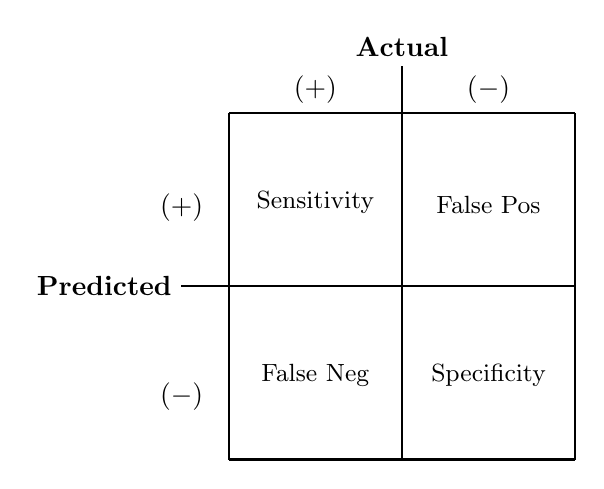
\begin{tikzpicture}[scale=2] %font=\scriptsize
    % Draw Basic Box
    \draw[thick] (0,0) -- (2.2,0);
    \draw[thick] (0,0) -- (0, 2.2);
    \draw[thick] (2.2,2.2) -- (2.2, 0);
    \draw[thick] (2.2,2.2) -- (0, 2.2);

    % Draw Box Ticks
    \draw[thick] (-0.3, 1.1) -- (2.2, 1.1);
    \draw[thick] (1.1, 0) -- (1.1, 2.5);

    % Box Labels
    % -- left side
    \coordinate[label=left:($+$)] (p1) at (-0.1,1.6);
    \coordinate[label=left:($-$)] (p2) at (-0.1,0.4);

    % -- top side
    \coordinate[label=above:($+$)] (p3) at (0.55, 2.2);
    \coordinate[label=above:($-$)] (p4) at (1.65, 2.2);

    % -- overall headers
    \coordinate[label=above:\textbf{Actual}] (p5) at (1.1, 2.5);
    \coordinate[label=left:\textbf{Predicted}] (p6) at (-0.3, 1.1);

    % Category Values
    \coordinate[label={\small{Sensitivity}}] (TP) at (0.55, 1.50);
    \coordinate[label={\small{False Pos}}] (FP) at (1.65, 1.50);
    \coordinate[label={\small{False Neg}}] (FN) at (0.55, 0.40);
    \coordinate[label={\small{Specificity}}] (TN) at (1.65, 0.40);
\end{tikzpicture}

\textbf{Receiver Operating Curve (ROC) / Area Under Curve (AUC)}

The ROC plots the true positive rate over the false positive rate at different classification thresholds. This generates a curve because when the threshold is 0, every prediction is positive, leading to a true positive rate of 1 and a false positive rate of 1. At the other extreme, when the threshold is set to 1, the false positive rate will be 0 and the true positive rate will also be 0.

A model which predicts randomly will produce an AUC value on an ROC plot of 0.5, and a perfect model which predicts correctly at every threshold would produce an AUC value of 1 (\cite{Aurélien2017} page 127). An AUC of 0 would be equivalent to 1 as the classification could be inverted.

\textbf{Conclusion}

The primary metric used to evaluate models in this project is the f1. Confusion matrices will also be used when providing further detail.

The selected metric must be applicable to both the iArsenic models and the machine learning based models. Because the iArsenic models do not provide a feature to change the classification threshold, a ROC cannot be produced. 

\section{Conclusion}

This chapter introduced existing prediction techniques used in related fields, including iArsenic which this project builds from, contextualised the application of these models with the black box problem, explored the possible tools available to implement and evaluate new models and explored which model types have been considered for development.

The following chapters include concepts detailed in this literature review, this chapter can be referred back to while reading further chapters.

The next chapter, Methodology, will outline exactly how these concepts have been researched and implemented throughout the development of this project. 
\chapter{Methodology}

This chapter will chronologically outline the steps planned and taken in the progression of the project.

The next chapter, Experiment Design, will detail how this methodology has been implemented.

At the start of the project, a high-level representation of the research and development steps required to complete the project was created as a Gannt chart. These steps were allocated a time frame and a sprint was planned at the start of each time frame.

This workflow is best described as a modified scrum methodology with a variable and flexible sprint window for each objective. Adherence to agile principles has guided decision-making when multiple options were available.

While each sprint was different, sprints broadly involved defining a clear goal and pursuing it until the end of the sprint window. While the sprint windows were not strict cut-offs, the primary focus of my time would change upon the start of a new sprint window.

The steps detailed in this chapter deviate from the initial plan specified in the Gannt chart. The changing project plan is inline with agile principles, embracing changing requirements and changing the plan as deemed necessary during reflection between sprints.

\section{Research Potential Projects}

The first step in this project was to identify potential project ideas. This was done with brainstorming, both by thinking about the project and talking about it with others.

The project ideas broadly fell into two categories, engineering, where the objective is to produce an application, and research, where the objective is to provide insight or an answer to an unknown.

A personal goal for me in this project was to develop my skills in machine learning and artificial intelligence. Evaluating the iArsenic models and producing alternative models with machine learning appealed to me as the most exciting project available. Because the project already contained a wealth of existing work, the objectives of this dissertation could build off this work instead of starting from scratch. This enabled higher level and higher impact objectives to be set. 

As Dr Mohammed Hoque agreed to be the client to this project I was able to commit to this project, confident in knowing it had purpose and direction from the client.

\section{Continuously Identifying Client Requirements}

In line with agile principles, the priority of this project was to satisfy the clients requirements. Therefore regular communications with Dr Hoque were prioritised in the form of emails and video calls where I would provide progress updates and Dr Hoque would provide feedback and direction. 

\subsection{Clarifying the Project Objectives}

Originally the vision of the project was to develop machine learning based models and compare their performance to the existing iArsenic models.

This initial vision is however does not define several key aspects of the project. How does one evaluate the performance of an iArsenic model? How does this compare to an evaluation of a machine learning based model? What is the purpose of developing new models and comparing them to the existing ones?

Ultimately the desired outcomes were clearly defined as the following:

\textbf{Desired Outcomes}

\begin{enumerate}
  \label{desired_outcomes}
  \item To evaluate the existing models
  \item To compare the performance of the existing models with typical machine-learning-based models
\end{enumerate}

Desired Outcome 1 was requested from the client. Evaluating the models informs the client of how each iteration of the models has impacted their performance and, because this model is deployed, verifies the quality of the predictions being made in deployment.  While the existing models were developed with expert knowledge, prior to the evaluations conducted in this project the performance of the iArsenic models was unknown.

The purpose of desired outcome 2 builds from the assertion made in \cite{Fleming2021} that machine learning should be part of Earth and Environmental Science. iArsenic provided an opportunity for a case study where expert system models can be compared to supervised learning models. 

\section{Research Applied Machine Learning Methodologies}

To design implement and evaluate machine learning models for iArsenic, I first had to research machine learning to understand what specific areas in machine learning could be applied to this dataset to achieve the desired outcomes of the project and then had to develop these models in code to gain the practical experience required.

Chapter 2 of \cite{Aurélien2017}, Hands-On Machine Learning with Scikit-Learn and TensorFlow, was the primary resource for breaking through the barrier of theoretical knowledge, gained from written sources such as \cite{Caruana2006} which compares several supervised machine learning models in different applications, to actually producing my own implementations of these models.

% TODO, could all the code in this section be moved to experiment design
\section{Understanding the iArsenic Code}

The iArsenic code provided the following key functions:

\begin{enumerate}
  \label{ia_functions}
  \item Producing a standard dataset
  \item Generating iArsenic models from a dataset
  \item Generating predictions from these generated models
\end{enumerate}

To learn how to achieve this functionality, I would read the iArsenic code in GitHub and experiment with it as an npm package.

\subsection{Producing a standard dataset}

The iArsenic script csv-to-json.js makes exporting a standardised dataset trivial.

This function is implemented in the project via an package script:

\begin{figure}[ht]
\begin{minted}[linenos, breaklines]{json}
"scripts": {
    "load-src-data": "mkdir well_data ; node node_modules/preprocessing/preprocessing/cli/csv-to-json.js -p node_modules/preprocessing/data/*.csv -o well_data/src_data.json",
\end{minted}
\label{fig:x load_ia_data}
\caption{Package.json snippet showing script to load data from iArsenic}
\end{figure}

\subsection{Generating iArsenic models from a dataset}

To verify that a model can generalise to new cases, it must be trained on a subset of the data and tested on a separate subset of data which it has not been previously exposed to, see \ref{eval} on page \pageref{eval}. In the iArsenic web application, the models are trained on the entire source dataset. See \ref{fig:x imp_iam_webapp} on page \pageref{fig:x imp_iam_webapp} for a flowchart showing this implementation.

Generating the iArsenic models from a training subset of the data was done by passing 4 of the 5 subsets of the data to the iArsenic model generator. This was done for each of the 5 subsets of the data for each of the 3 iArsenic models. See \ref{fig:x programmatically_gen_ia_model} on \pageref{fig:x programmatically_gen_ia_model} to see the code that achieved this.

\begin{figure}[ht]
    \centering
    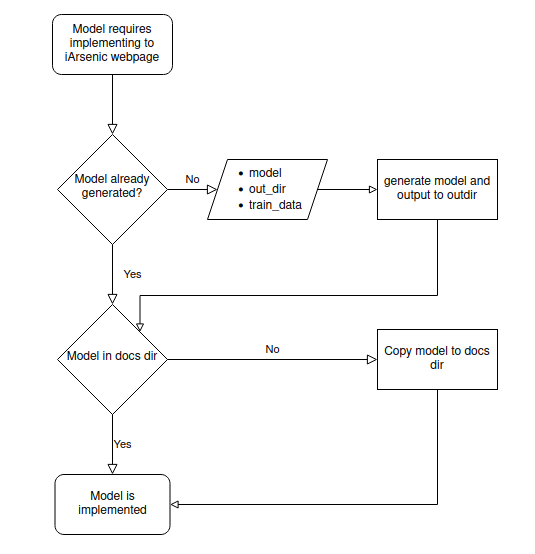
\includegraphics[scale=0.6]{figures/implement_ia_model_to_webapp.png} 
    \caption{Flowchart showing process to implement model in iArsenic webapp}
    \label{fig:x imp_iam_webapp}
    \small The code that generates the models can be found at: \url{https://github.com/portsoc/iArsenic/blob/master/preprocessing/cli/produce-aggregate-data-files.js}
\end{figure}

\begin{figure}[h]
    \begin{minted}[linenos, breaklines]{python3}
def gen_model(train_src, out_dir, model):
  if not os.path.exists(out_dir):
    os.mkdir(os.path.join(out_dir))

  cmd = [
    'node',
    'node_modules/preprocessing/preprocessing/ cli/produce-aggregate-data-files.js', 
    '-m',
    model,
    '-o',
    out_dir,
    '-p',
    train_src,
    'node_modules/preprocessing/data/mouza-names.csv',
  ]
  stdout = check_output(cmd).
    decode(sys.stdout.encoding).
    replace('\n', '')
    
  print(stdout)
    \end{minted}
    \caption{Python code used to programmatically generate iArsenic models. In iArsenic this is done via the command line}
    \label{fig:x programmatically_gen_ia_model}
    \small The file containing this code can be found at: \url{https://github.com/JavaRip/UoP-SoftEng-Dissertation/blob/main/models/model_utils/gen_ia_model.py#L9-L25}
\end{figure}

\subsection{Generating predictions from generated iArsenic models}

The web application index.html file shows a script.js file is used, in this file a global function called produceEstimate is called from the estimator.js script. See \ref{fig:x produce_estimate_call} on \pageref{fig:x produce_estimate_call} to see this function call.

\begin{figure}
    \begin{minted}[linenos, breaklines]{python3}
    const estimate = produceEstimate(aggregateData, inputs.division, inputs.district,
      inputs.upazila, inputs.union, inputs.mouza, inputs.depth, inputs.colour, inputs.utensil, inputs.flooding);
    \end{minted}
    \caption{Code used in iArsenic to produce estimate from a model in the webapp}
    \label{fig:x produce_estimate_call}
    \small The file containing this code can be found at: \url{https://github.com/portsoc/iArsenic/blob/master/docs/script.js#L340-L341}
\end{figure}

\section{Developing New Models}

To familiarise myself with implementing machine learning models, I initially followed the tutorial in Chapter 2 of \cite{Aurélien2017}'s book Hands-On Machine Learning with Scikit-Learn. I then implemented 4 separate supervised learning models on 25 datasets from the internet, see \ref{fig:x 4_m_25_d}. This was to develop my skills, in line with the agile principle continuous attention to technical excellence.

\begin{landscape}
    \begin{figure}[ht]
        \centering
        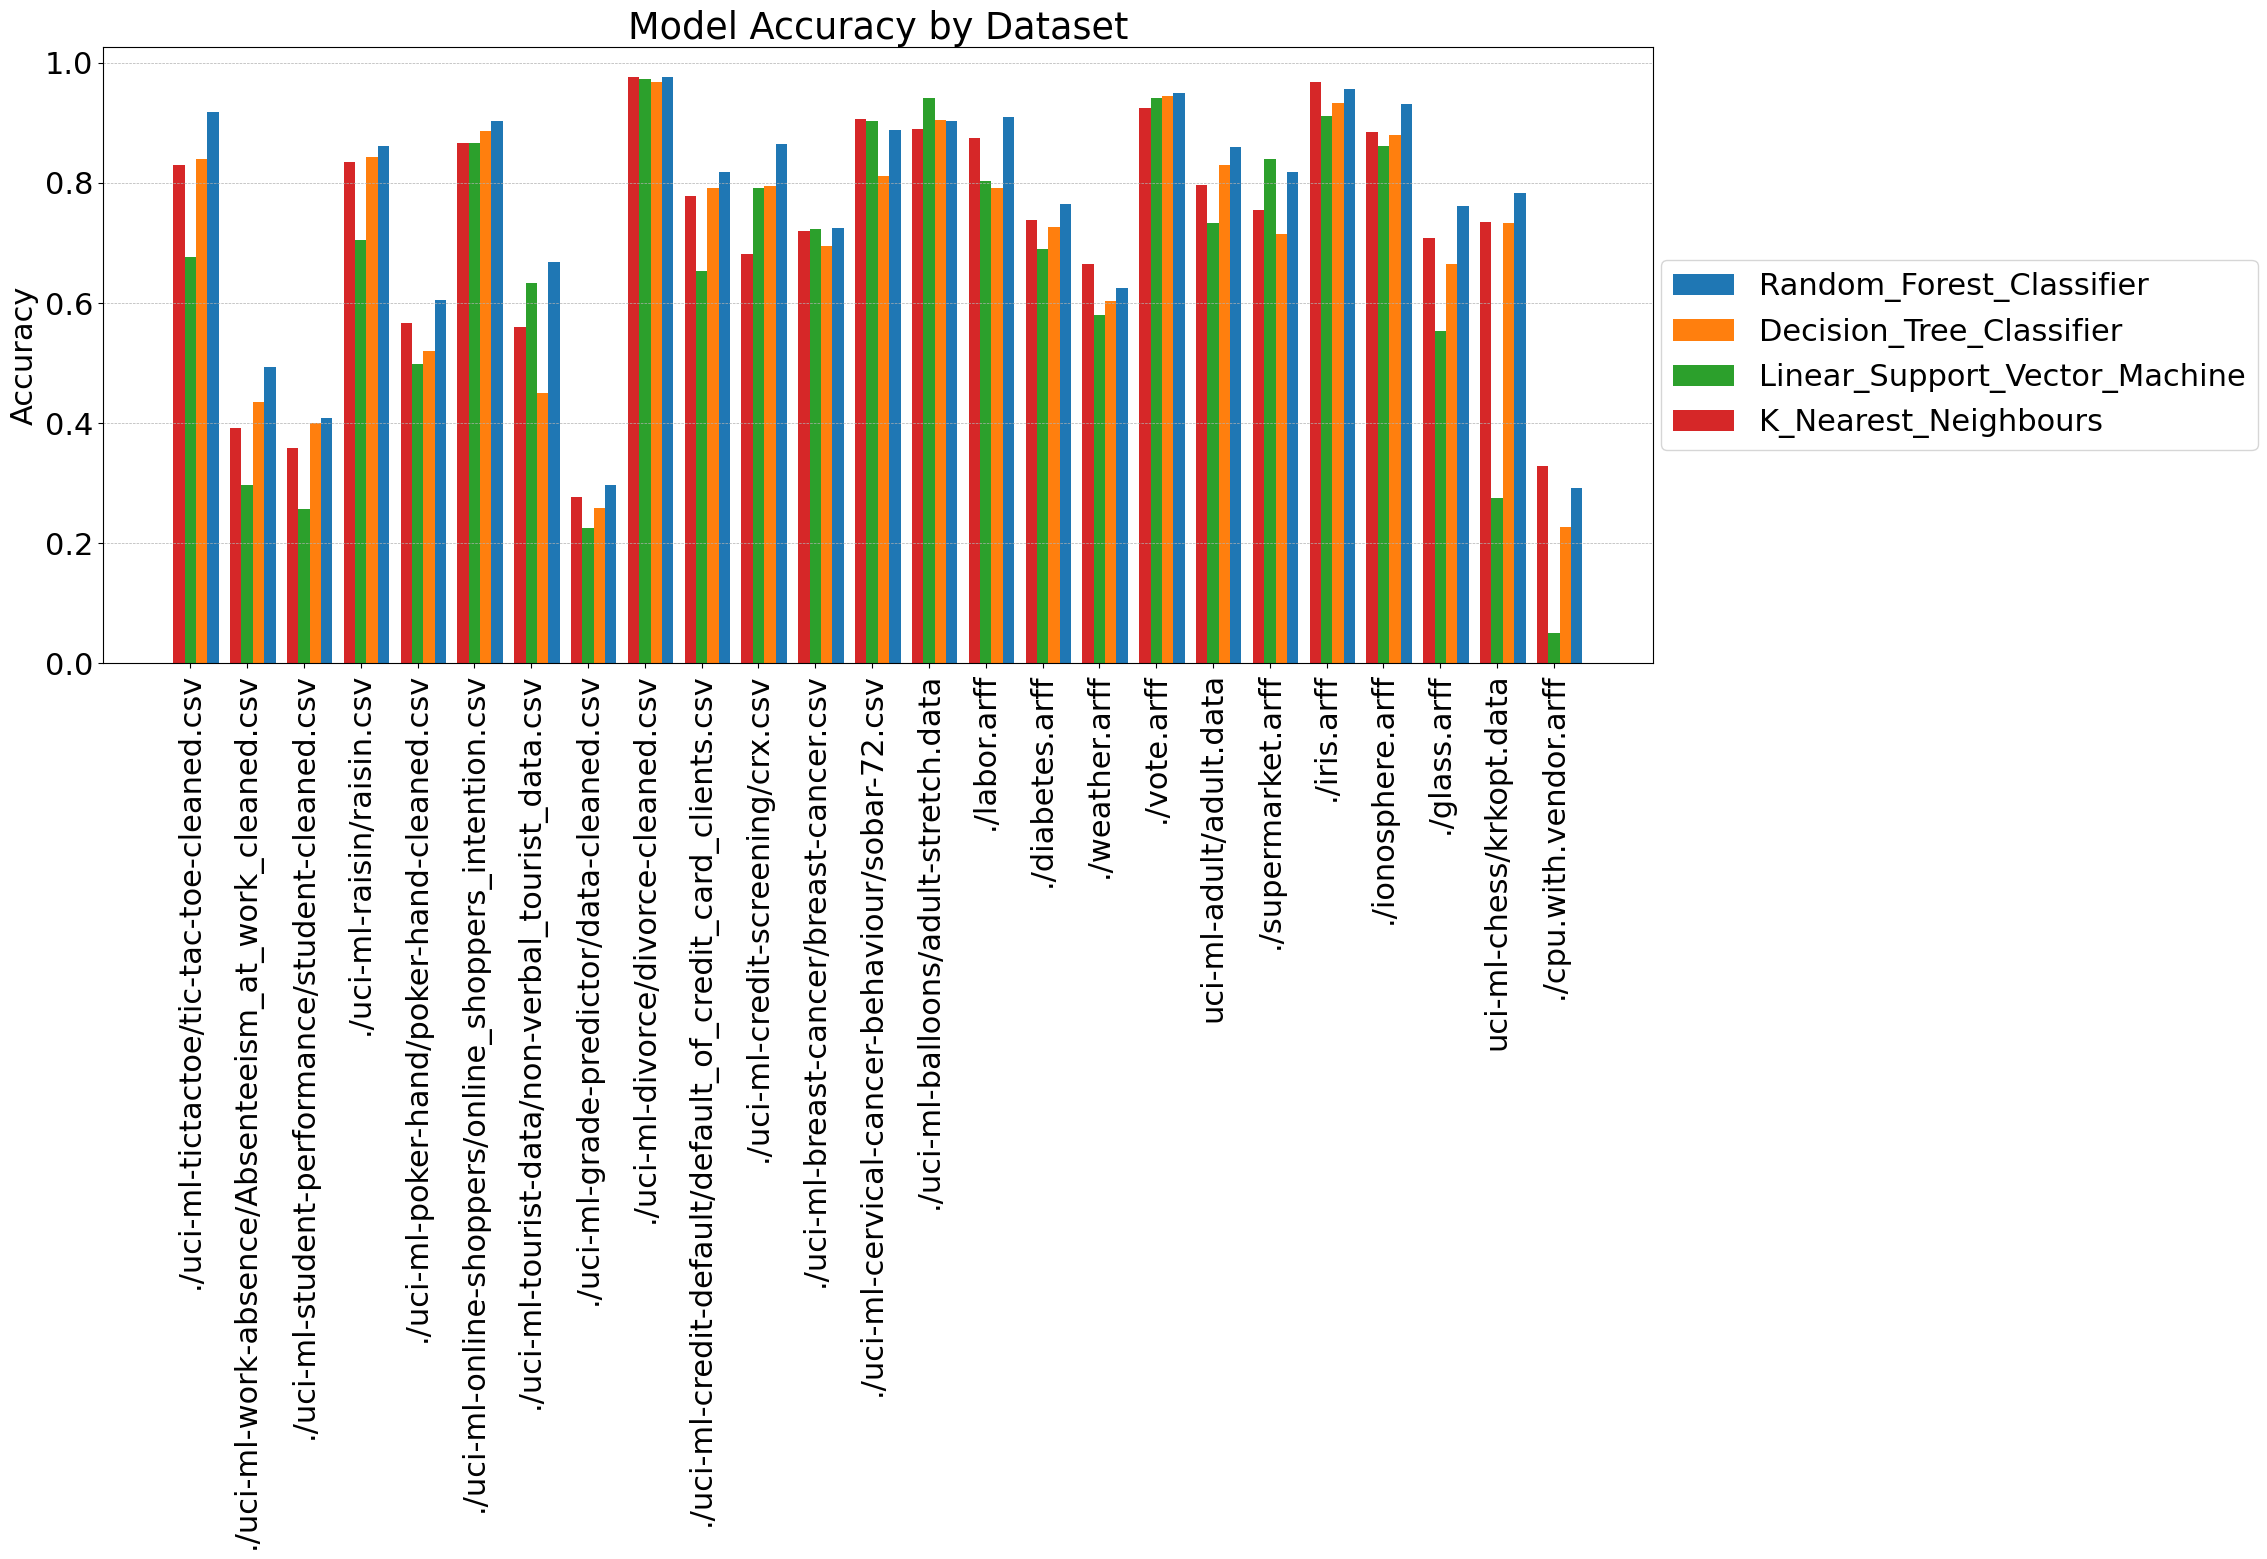
\includegraphics[scale=0.375]{figures/4_models_25_datasets.png} 
        \caption{Summary of results of supervised model implementation practice}
        \label{fig:x 4_m_25_d}
    \end{figure}
\end{landscape}

\section{Integrating iArsenic and scikit-learn}

The prototype implementations of both iArsenic and machine learning based models allowed each model to take input data and produce estimations individually. 

Because it takes multiple days to run every experiment required, it is not practical to have a human run each model individually. The time between an experiment finishing and the next starting will depend on when the human gets around to it. By making the models run programmatically this is not an issue. It also makes the project to be more portable, allowing it to be run on a remote server or high performance computer.

To run both NodeJS based iArsenic models and Python based scikit-learn models an integration layer between Python and NodeJS had to be created. Python was chosen as the main program to run the NodeJS code from as a personal preference. Using NodeJS would also have been a reasonable choice. See \ref{fig:x ia_model_sd} on page \pageref{fig:x ia_model_sd} to see the flow of data from the main.py script to the iArsenic models to produce estimates for a test dataset.

\begin{figure}
    \centering
    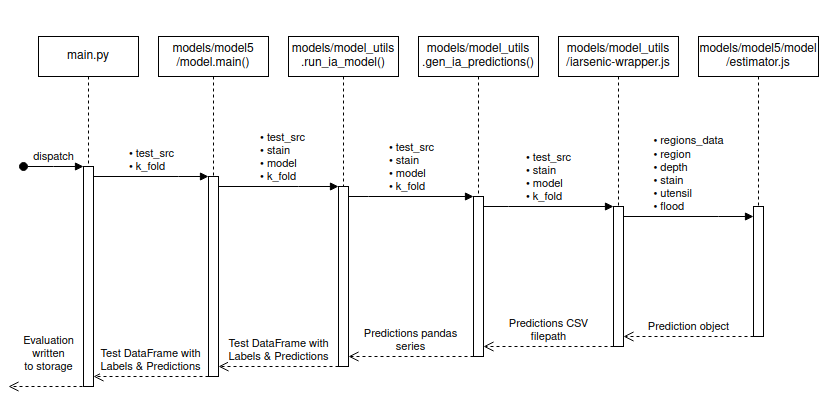
\includegraphics[width=\textwidth]{figures/ia_model_sd.png} 
    \caption{Sequence diagram showing Python to NodeJS variable bridge over storage}
    \label{fig:x ia_model_sd}
\end{figure}

\section{Main Project Structure}

The project architecture has a top-level main file, which when run will produce an evaluation for each model. See \ref{fig:x p_fs} on page \pageref{fig:x p_fs} to see the file structure of the project.

This structure combined with the requirement for the models to be run programmatically, facilitates continuous delivery of new models. Conforming to the agile principle of delivering working software frequently.

\begin{figure}
    \begin{minted}[]{bash}
|-- evaluation_data/    # model performance metrics
|-- experiments/        # ad-hoc experiments
|-- geodata/            # uncompressed geodata
|-- geodata.zip
|-- main.py             # prediction & evaluation generation entry point
|-- models/             # all models to be run go in here
    |-- model{number}/  # model entry point & model dependencies
        |-- model.py    # takes test CSV & k-fold, returns predictions
    |-- model_utils/
|-- package.json	
|-- package-lock.json	
|-- prediction_data/    # test CSVs with predictions & labels by model
|-- requirements.txt
|-- utils/		
|-- well_data/          # iArsenic standard dataset
    \end{minted}
    \caption{Project file structure}
    \label{fig:x p_fs}
\end{figure}

\section{Conclusion}

The distinction between leadership and production in \cite{Covey2013} on pages 98 to 99 explains the difference between this chapter and the next. 

This chapter outlines how the work is going to be done, including specifying the purpose of the project and developing the knowledge and software architecture required to produce the experiments required to achieve the desired outcomes, the next chapter Experiment Design, outlines how this plan will be implemented.

This chapter described the leadership and management, the next chapter describes the production.
\chapter{Experiment Design}

This chapter defines how the desired outcomes defined in the Methodology chapter will practically be met. This requires describing the available code and data, how it will integrate with new code developed in this project and what the new code being developed is.

This chapter also details how the existing work in iArsenic is utilized.

\section{Well Data in iArsenic}

The data used by iArsenic can be found in the CSV in the data/ directory of iArsenic (note that this does not include CSV files in sub-directories of the data/ directory). These files have been selected on the following criteria for aggregating:

\begin{itemize}
    \item two CSV files do not include the same datapoint
    \item the CSV contains standard features required by the iArsenic models
\end{itemize}

Before preprocessing, these files contain 1,144,586 rows (including headers) combined.

The primary preprocessing function provided by iArsenic is applying name corrections. This is the process of changing region names such that a region with inconsistent naming in source data files, has the same name in an aggregate dataset. These corrections allow the well data and the geodata to be aggregated.

After preprocessing, the iArsenic data contains 868,678 rows (excluding headers). 475,182 data points are negative (safe/equal to or below 10µg/l), and 393,496 are positive (polluted / above 10µg/l), the null positive rate (the accuracy when always predicting false) is 55\%. The name corrected dataset output by iArsenic will be referred to as the iArsenic Standard Dataset.

See figure \ref{fig:x avg_datapoints} on page \pageref{fig:x avg_datapoints} for a choropleth of datapoints per District.

For a more detailed summary of the data, see table \ref{tbl:x reg_size_dp} on page \pageref{tbl:x reg_size_dp} to see the region sizes and datapoints per region.

\begin{figure}[!htb]
    \centering
    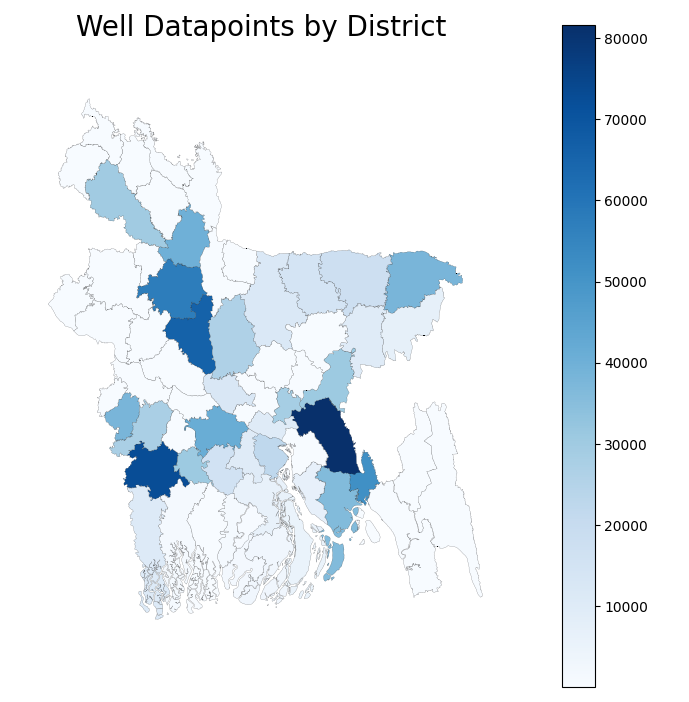
\includegraphics[scale=0.57]{figures/data_distribution_by_district.png} 
    \caption{Distribution of Well Data by District in iArsenic Standard Dataset}
    \label{fig:x avg_datapoints}
\end{figure}

\newpage

The attributes included in the iArsenic standard dataset file are the following:

\begin{itemize}
    \item Division
    \item District
    \item Upazila
    \item Union
    \item Mouza
    \item Depth
    \item Arsenic
\end{itemize}

Excluding Depth and Arsenic, attributes are region names with corresponding geographic data.

See figure \ref{fig:x labelled_divisions} on page \pageref{fig:x labelled_divisions} for a labelled map of Bangladesh divisions.

\begin{table}
    \centering
    \begin{tabular}{c c c c c c} 
         \toprule
         Name & Mean Area $km\textsuperscript{2}$ & Area $\sigma$ & Mean Data & Data $\sigma$ & Unique Values \\ 
         \midrule 
         Division & 17,482 & 6,928 & 108,584 & 72,085 & 8 \\ 
         District & 2,185 & 1,080 & 13,788 & 20,102 & 63 \\
         Upazila & 257 & 185 & 1,952 & 5,683 & 445 \\
         Union & 27 & 41 & 306 & 786 & 2,838 \\
         Mouza & 2.4 & 8.4 & 90 & 191 & 9,550 \\
         \bottomrule
    \end{tabular}
    \caption{Region sizes, datapoints per region \& count}
    \label{tbl:x reg_size_dp}
\end{table}

\begin{figure}
    \centering
    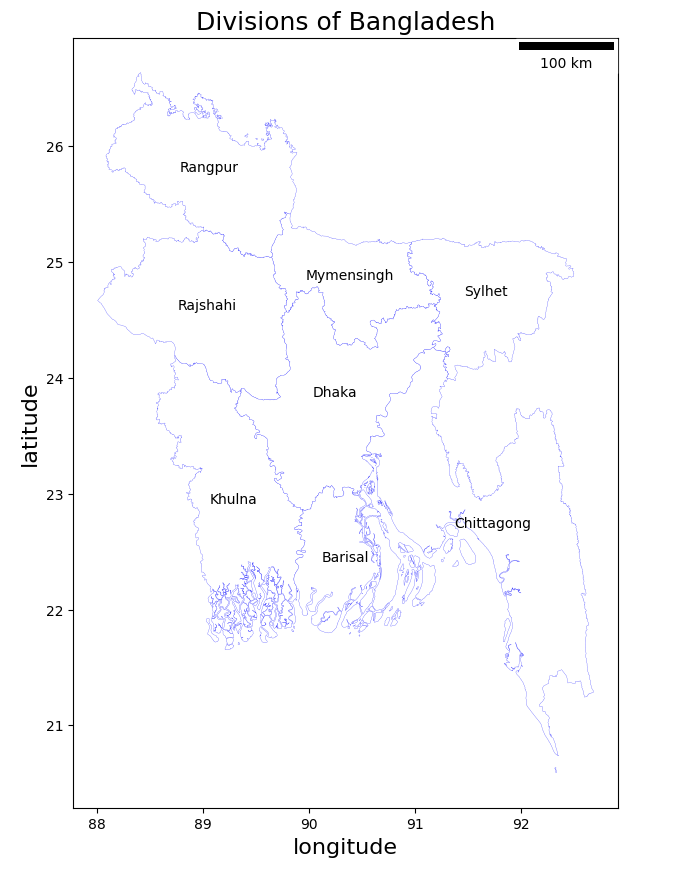
\includegraphics[scale=0.45]{figures/labelled_divisions.png} 
    \caption{The Divisions of Bangladesh mapped and labelled}
    \label{fig:x labelled_divisions}
\end{figure}

\textbf{Depth}

The Depth column refers to the depth of a well in meters.

The deepest well in the dataset is 445 meters, the lowest is 0, the is mean 40 meters and the standard deviation is 52 meters. See figure \ref{fig:x avg_depth} on page \pageref{fig:x avg_depth} for a choropleth of mean depth per Upazila and \ref{fig:x dva} on page \pageref{fig:x dva} so see the relationship between mean depth and mean arsenic by division.

\begin{figure}[!htb]
    \centering
    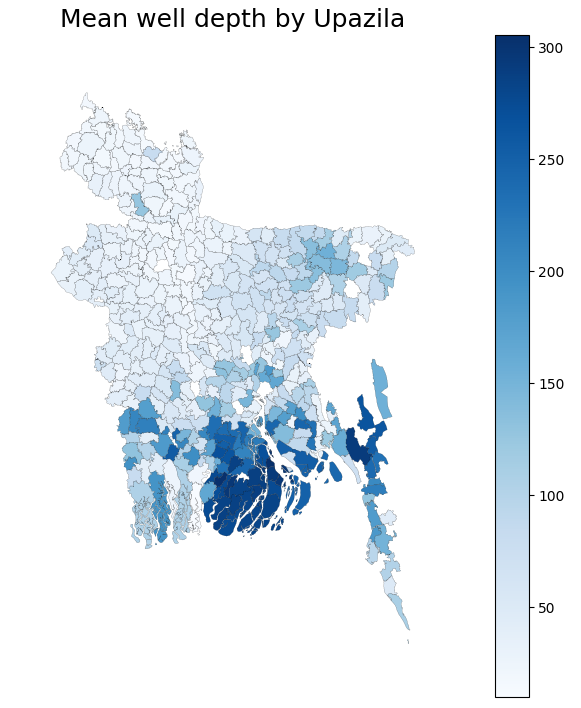
\includegraphics[scale=0.54]{figures/mean_well_depth_by_upa.png} 
    \caption{Average (mean) Well Depth by Upazila}
    \label{fig:x avg_depth}
\end{figure}

\begin{figure}[!htb]
    \centering
    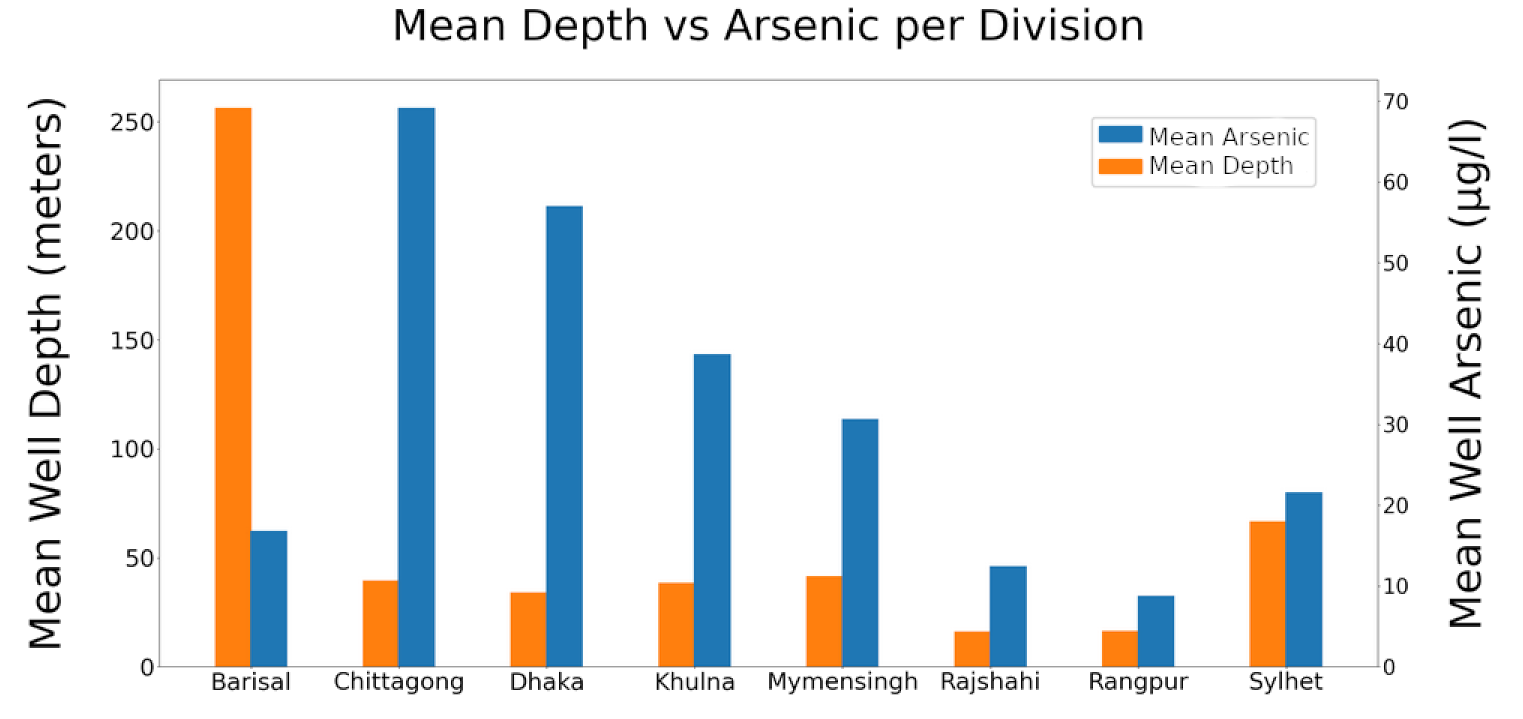
\includegraphics[scale=0.28]{figures/mean_as_vs_depth.png} 
    \caption{Chart showing the relationship between mean well depth and arsenic pollution}
    \label{fig:x dva}
\end{figure}

\textbf{Arsenic}

The Arsenic column refers to the arsenic concentration in water from a well datapoint in micro-grams per litre ($\mu$g/l).

The highest concentration of arsenic in the iArsenic standard dataset is 4,000$\mu$g/l (4ng/l), the lowest concentration of arsenic is 0$\mu$g/l, the mean is 41$\mu$g/l and the standard deviation is 74$\mu$g/l. See figure \ref{fig:x avg_as} on page \pageref{fig:x avg_as} for a choropleth of mean depth per Upazila.

\begin{figure}[!htb]
    \centering
    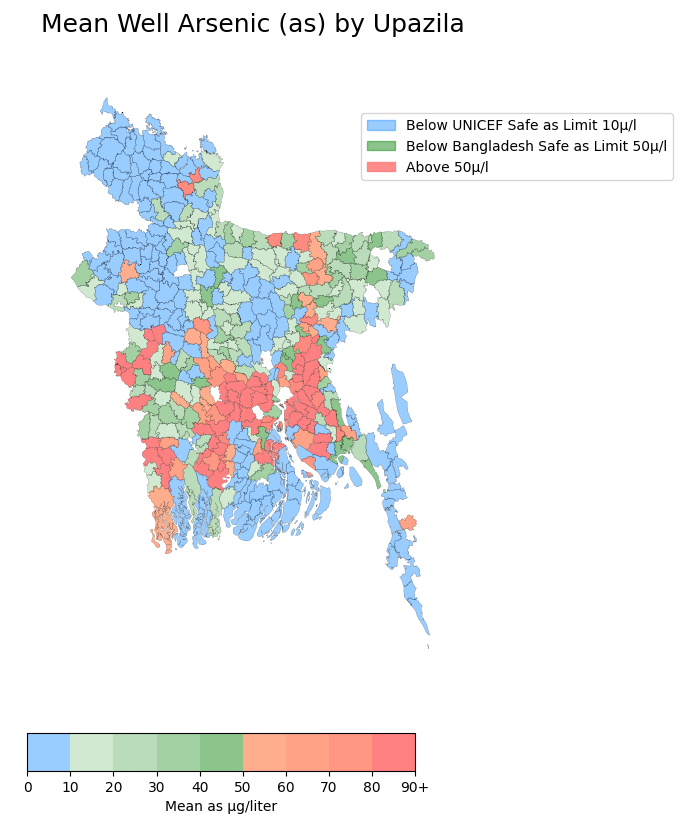
\includegraphics[scale=0.6]{figures/mean_as_by_upazila.png} 
    \caption{Distribution of Average (mean) Arsenic by Upazila in the iArsenic Standard Dataset}
    \small{See page \pageref{fig:x avg_as_cblind} for a red-green colorblind compatible version of this diagram}
    \label{fig:x avg_as}
\end{figure}

\newpage

\textbf{Why use this Dataset?}

While new and existing iArsenic models could be trained on different data, the time and resources required to produce a dataset of this quality and suitability are substantial and outside the scope of this project. 

\subsection{Geodata}

The original source of the geodata is unclear, though similar country-based polygon data can be found on the first page of Google.

The geodata has been zipped and added to the project's repository using Git Large File Storage. This is because some of the geodata are omitted from the original iArsenic repository due to it exceeding the GitHub file size limit. 

Instructions are provided in iArsenic for regenerating this missing data at the following url: \url{https://github.com/portsoc/iArsenic/tree/master/preprocessing/geodata}

\section{iArsenic Integration}

\subsection{Data Preparation}
\label{sub: data_prep}

The iArsenic code repository is downloaded from GitHub via Node Package Manager (npm). This repository includes selected source data and several tools to process this data.

Data is extracted from iArsenic using the csv-to-json.js script. This script aggregates the source files into a single data structure and outputs it as a JSON file. Additionally, it ensures that all regions follow the same naming convention, which is essential because it prevents distinct data points in the same region from appearing to be in two different regions. This enables the data to be matched to its corresponding polygon in the geodata.

The JSON file is then converted to a pandas DataFrame in Python, shuffled to ensure there is no ordering bias, and converted into 5 separate CSV files. It is split into 5 to enable k-fold cross-validation on the dataset.

These 5 CSV files are what we use to test and train the models.

See the script that generates the 5 data subsets here: \url{https://github.com/JavaRip/UoP-SoftEng-Dissertation/blob/main/utils/src_to_test_train.py}

\subsection{Generating the iArsenic Models}

iArsenic can generate 3 separate models: model3, model4 and model5.

Originally an iArsenic model was generated on all available data and then made available on the iArsenic web application. Due to their modular design, however, the models can also be imported into NodeJS.

To evaluate the models using k-folds cross-validation, each of the 3 models is generated 5 times with 4 of the CSVs used for training and 1 for testing, thus implementing k-folds cross-validation. This requires generating a total of 15 iArsenic models.

\subsection{Interfacing With Generated iArsenic Models}

Predictions are generated from the generated model using a NodeJS script. This will be referred to as the iArsenic Model Wrapper.

The predictions are saved to a temporary CSV file and the name of this file is logged to the standard output.

The iArsenic model wrapper requires the following parameters to be passed as system arguments:
\begin{itemize}
  \item a CSV file containing the data points to use to generate predictions
  \item the stain colour of the well the data point is from
  \item the model to generate the prediction from
  \item the k-fold version of the model to generate the prediction from
\end{itemize}

Initially, the iArsenic Wrapper Script would produce an estimate from one data point at a time, passed as a system argument. However, this would take days to pass the every datapoint in the test dataset. Therefore the test dataset is passed as a CSV file path, which takes less than an hour to process.

\subsection{Imputing Stain Colour}

In the original iArsenic web application, the stain colour was to be specified by a user entering parameters about a real well, requiring the user to observe and provide the staining colour of the well. The data extracted from iArsenic however did not include staining colour data. 

When working with missing values there are primarily 3 options (see \cite{Aurélien2017} page 88): 

\begin{enumerate}
    \item remove the feature with missing values
    \item delete all rows containing missing data
    \item replace missing data with a fixed value
\end{enumerate}

Because the iArsenic models will not run with the colour omitted, option 1 is not viable. Because none of the rows contain staining data, option 2 is also not viable. Therefore we must fill in the data with a fixed value, either 'Red' or 'Black'.

To determine whether the value should be set to 'Red' or 'Black', the models have been evaluated using each and the value with which the model performs best, 'Red', has been selected. Figure \ref{fig:x ia_model_black_red_accuracy} on page \pageref{fig:x ia_model_black_red_accuracy} shows the accuracy of the iArsenic models with 'Black' or 'Red' used as the imputed well colour.

\begin{figure}[h]
    \centering
    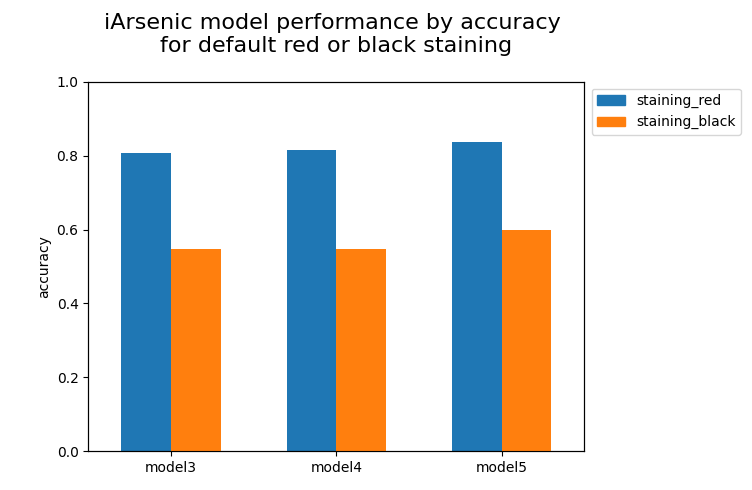
\includegraphics[scale=0.55]{figures/ia_model_black_red_accuracy.png} 
    \caption{iArsenic model performance by accuracy for default red vs black staining}
    \label{fig:x ia_model_black_red_accuracy}
\end{figure}

\newpage

Considering the accuracy score alone, it appears that setting the parameter to 'Red' produces the best model performance by approximately 20\%. As mentioned in \cite{EM} on page \pageref{EM}, a higher accuracy score however does not guarantee that one model outperforms another.

Comparing the sensitivity and specificity of the models shows that when the staining is set to 'Black' model3 and model4 always assume the well is safe. The sensitivity, the true positive rate, becomes 0 and the specificity, the true negative rate, becomes 1. While the specificity is lower when the staining is set to 'Red', the sensitivity is much higher for each model, indicating better performance. See \ref{fig:x ia_svs_red} on page \pageref{fig:x ia_svs_red} for the sensitivity and specificity plotted as a bar chart for 'Red' and 'Black staining for comparison.

\newpage

\begin{figure}[!htb]
    \centering
    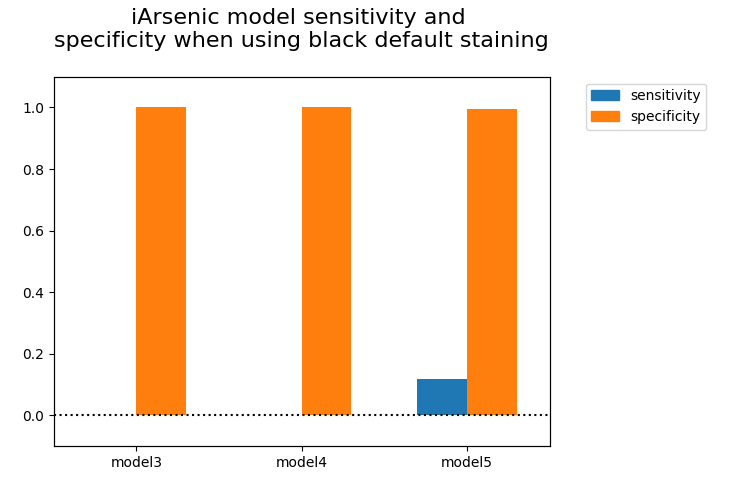
\includegraphics[scale=0.55]{figures/ia_models_sensitivity_vs_specificity_black.png} 
    \label{fig:x ia_svs_black}

    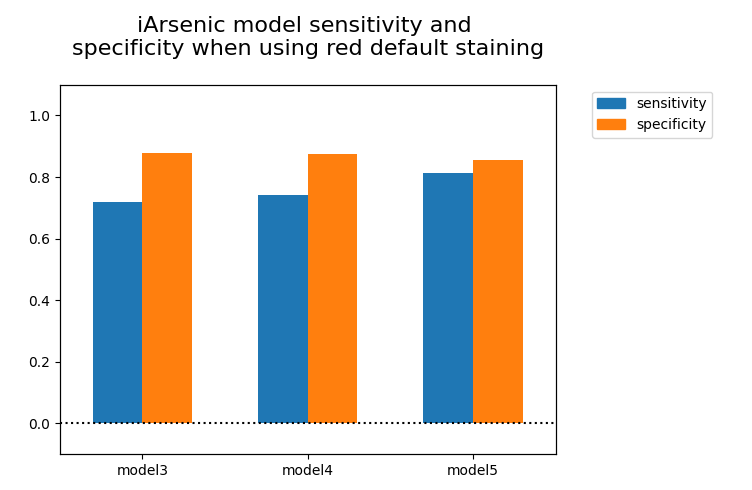
\includegraphics[scale=0.55]{figures/iarsenic_model_sensitivity_vs_specificity_red.png} 
    \caption{Model sensitivity and specificity stain parameter 'Black' (top) vs 'Red' (bottom)}
    \label{fig:x ia_svs_red}
\end{figure}

\newpage

Generating two confusion matrices for model5, one generated from 'Black' passed as a parameter and one from 'Red', reinforces the conclusion that using 'Red' as a parameter produces a better model. See \ref{fig:x Confusion Matrix mode5 Red Staining} on page \pageref{fig:x Confusion Matrix mode5 Red Staining} to see a confusion matrix for each staining parameter for comparison of evaluations.

\begin{figure}[!htb]
    \centering
    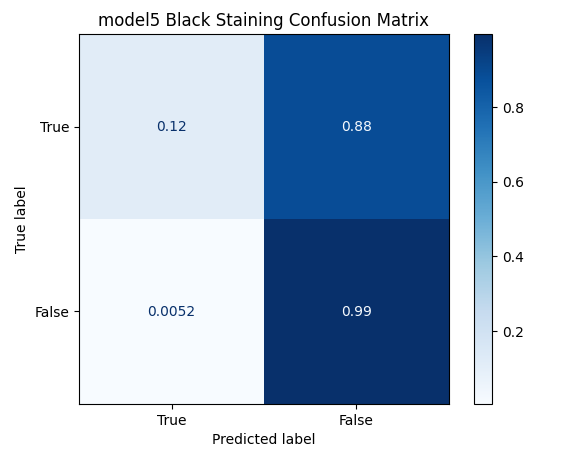
\includegraphics[scale=0.6]{figures/m5_black_cm.png} 
    \label{fig:x Confusion Matrix mode5 Black Staining}
    
    \centering
    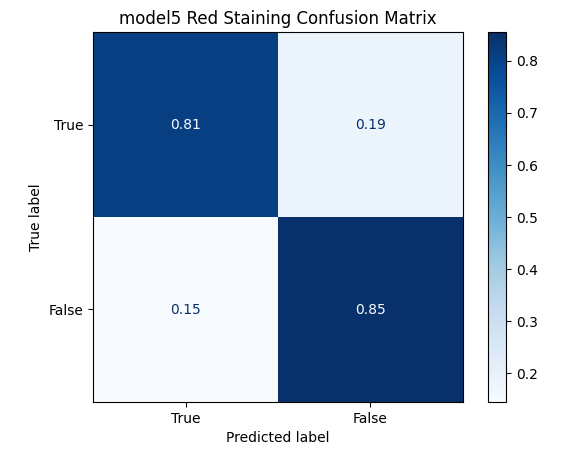
\includegraphics[scale=0.6]{figures/m5_red_cm.png} 
    \caption{Confusion Matrix model5 'Black' (top) vs 'Red' (bottom) Staining}
    \label{fig:x Confusion Matrix mode5 Red Staining}
\end{figure}

\newpage

\textbf{Quantitative Approach to Selecting Staining Parameter}

Observing the evaluation metrics of the iArsenic models and comparing them when producing predictions with either 'Red' or 'Black' as the staining parameter has indicated that the models perform better with 'Red' passed as a parameter. This is however still arguably down to interpretation.

A quantitative comparison of the models, using a value such as area under the curve would be a beneficial addition to the evaluation. This however is not possible with the iArsenic models as there is no feature to change the classification threshold, which is required to generate a receiver operating curve and therefore calculate the area under the curve.

\section{Creating a Common Model Interface}

The machine learning models will be made in Python. These can be interfaced with directly using Python modules with parameters passed directly into function calls. This is inconsistent with the iArsenic models which are run via the iArsenic Wrapper Script using node, passing parameters with command line arguments.

A Common Module Interface has therefore been specified which standardises how the modules should be interacted with. This interface specifies that each model will have a main function which takes two parameters, the test data source and the k-fold number, and returns predictions as a pandas DataFrame.

\subsection{Implementing the Common Model Interface}

Each model has a directory in the top-level models directory. Each model directory contains a model.py file which exports a Python module which can generate predictions based on the Common Module Interface, in addition to any other resources required by the model. See \ref{fig:x p_fs} on page \pageref{fig:x p_fs} for an illustration of this file structure.

Because it is a NodeJS script, the iArsenic Model Wrapper cannot accept variables passed by Python. Therefore a Python to NodeJS Bridge has been created. The Python to NodeJS Model Bridge works by running the iArsenic Model Wrapper from Python in a subprocess managed by Python from the main.py script.

\section{Evaluating the Models}

The predictions returned from the common model interface are used for evaluation. The following evaluation metrics are generated:
\begin{itemize}
  \item accuracy
  \item sensitivity 
  \item precision 
  \item specificity 
  \item f1
\end{itemize}

See \ref{EM} on page \pageref{EM} for a detailed explanation of these metrics.

\subsection{Standardizing Classifications}

The iArsenic models generate predictions from 1 of three classifications, safe, polluted, highlyPolluted. The scikit-learn models could be configured to output any number of classifications.

To adhere to conventional evaluation metrics the iArsenic predictions were simplified to safe or polluted, where highlyPolluted predictions are converted to polluted. This enables the metrics detailed in \ref{EM} on page \pageref{EM} to be used instead of defining our own evaluation methods and metrics, which would be less comparable to other real-world models.

\section{Creating a Main Script to Run \& Evaluate Experiments}

The Common Module Interface allows the models imported to the main.py script and run programmatically, without specific code defined for each model. 

This facilitates maintainable code as the complexity of the code increases. The complexity of the main.py script necessitates that steps to ensure maintainability are taken. 

Significant complexity has been introduced in making the models run and build concurrently. This is important however as doing this sequentially would take more time than is practical.

The iArsenic models benefit the most from being run concurrently as these are single-threaded. Running them concurrently allows more of the host machine's CPU power to be utilised by using multiple CPU cores simultaneously.

The machine learning models however are written using scikit-learn libraries, which are able to use all CPU cores available. 

Further optimizing the models by, for example, running the iArsenic models concurrently and the machine learning models sequentially was not deemed necessary, as building and running all models concurrently took approximately 3.5 days, which is a practical amount of time. This run was achieved on a server computer with Ubuntu 22.01, an 8 x 1.8GHz core CPU and 96GB 1600MHz DDR3 RAM.

\subsection{Main Script Structure}

The purpose of the main.py script is to provide an entry point to execute all required steps of the project.

The main script takes the following steps:
\begin{enumerate}
    \item extract the iArsenic \& geodata
    \item generate the k-folds cross-validation data split 
    \item build the iArsenic models
    \item generate predictions from all models
    \item generate an evaluation for each model's predictions
\end{enumerate}

\section{Development of New Models}

In the existing work section of the literature review \ref{ew} on page \pageref{ew}, 3 model approaches were examined.

The iArsenic models implement elements of k-nearest neighbour algorithms, \cite{Winkel2008} used random forests. This makes these model types candidates for further experimentation. Multilayer feed-forward neural network classifiers are also used because of their versatility in machine learning.

The models in both \cite{Winkel2008} and \cite{Connolly2022} ues latitude and longitude. Because of the availability of geodata in this project, preprocessing regions to their latitude and longitude is considered a viable technique. 

The iArsenic models calculate global variables during preprocessing, including the lower quartile, upper quartile and median arsenic concentrations for any given region. This processed data can be extracted from the iArsenic model and passed to a machine-learning model.

Another preprocessing technique used is applying no preprocessing.

When initially developing a model, intuition is used to hypothesize how a model might potentially work. After being implemented in code it is optimized. Neural networks have required substantial optimizations to allow the models to be trained and produce predictions within hours instead of days or weeks, at the compromise of model performance.

The predicted suitability of these model types is reinforced by \cite{Caruana2006} when comparing the performance of machine learning algorithms over different types of datasets.

\subsection{Summary of Models and Preprocessing Techniques Implemented}

\textbf{Types of Model}

\begin{enumerate}
    \item K-Nearest Neighbours Classifier
    \item Random Forest Classifier
    \item Multilayer Perceptron Feed Forward Neural Network Classifier
\end{enumerate}

\textbf{Types of Preprocessing}

\begin{enumerate}
    \item No preprocessing
    \item Conversion of region names to latitude and longitude
    \item Extracting iArsenic model preprocessed data
\end{enumerate}

\subsection{model6}

Model6 is an implementation of scikit-learn's random forest classifier with the default configuration.

Because this model cannot process string values, all string values are converted to numerical values, with each new string given an identification number in ascending order.

No preprocessing is applied to the data.

\subsection{model7}

Model7 is also a default implementation of scikit-learn's random forest classifier. This model incorporates computed region attributes computed in model5.

model5 uses feature engineering to calculate the median, lower quartile and upper quartile of the arsenic in a region, for a given depth range.

The hypothesis is that this feature engineering will provide the model with information that correlates with the model prediction target for a given data point, improving the models performance.

These values are therefore incorporated into the dataset used for model7. Where the values for a region are missing from the model5 dataset, the values from the region's parent are used.

\subsection{model8}

Model8 uses a feed-forward neural network, scikit-learn's MultiLayer Perceptron Classifier (MLPClassifier) model. See the configuration of model8 in table \ref{tbl:x m8_config} on page \pageref{tbl:x m8_config}.

\textbf{Neural Network Configuration}

\begin{table}
    \centering
    \begin{tabular}{c c c c c} 
         \toprule
         Hidden Layers & Solver & Learning Rate & Epochs & Validation \\ [0.5ex] 
         \midrule
         3 & adam & adaptive & 100 & 10\% of train\\ 
         \bottomrule
    \end{tabular}
    \caption{Model8 MLP configuration}
    \label{tbl:x m8_config}
\end{table}

The first hidden layer consists of half the number of inputs, the next hidden layer one-quarter the number of inputs and the final hidden layer one-eighth. The adam algorithm is used because it is generally faster than standard gradient descent on datasets this size. An adaptive learning rate is used to allow the performance to increase up to the maximum limit of 100 epochs.

\textbf{Data Preprocessing \& Feature Engineering}

The median, upper quartile and lower quartile arsenic values are imported from the model5 processed data to the dataset used by this model.

The smallest region size, the Mouzas are one hot encoded, allowing each Mouza to have a corresponding input node.

The region columns are dropped.

The data is normalised between 0 and 1.

\textbf{Model Optimization}

Due to the number of Mouzas (9550), the model could not allocate enough memory to run with the source data passed directly.

Therefore the source data has been split into 8 subsets by Division (See figure \ref{fig:x labelled_divisions} on page \pageref{fig:x labelled_divisions}. For each Division a model is trained with the data points within that region and predictions are generated. These predictions are then added to their corresponding data points in the source dataset.

The implementation of this optimization can be seen in figure \ref{fig:x m8_code} on page \pageref{fig:x m8_code}.

\begin{figure}[h]
    \begin{minted}[linenos]{python3}
  for div in train_df['Division'].unique():
    tr_div = train[train['Division'] == div]
    te_div = test[test['Division'] == div]
    
    tt_df = append_test_train(te_div, tr_div)
    
    conv_cat_num(tt_df, 'Label')
    tt_df = ohe_col(tt_df, ['Mouza'])
    
    tt_df = tt_df.drop(
      columns=[
        'Division',
        'District',
        'Union',
        'Upazila',
      ]
    )
    
    cat_int_enc(tt_df)
    tt_df = pd.DataFrame(
      MinMaxScaler().fit_transform(tt_df), 
      columns=tt_df.columns
    )
    
    te_div, tr_div = split_test_train(tt_df)
    
    train_X = tr_div.drop(['Arsenic', 'Label'], axis='columns')
    train_y = tr_div['Label']
    test_X = te_div.drop(['Arsenic', 'Label'], axis='columns')
    
    num_feat = len(test_X.columns)
    
    clf = MLPClassifier(
      solver='adam',
      alpha=0.0001,t
      hidden_layer_sizes=(
        math.trunc(num_feat / 2), 
        math.trunc(num_feat / 4), 
        math.trunc(num_feat / 8)
      ),
      learning_rate='adaptive',
      random_state=99,
      max_iter=100,
    )
    
    clf.fit(train_X, train_y)
    
    test.loc[test['Division'] == div, ['Prediction']] = clf.predict(test_X)
    \end{minted}
    \caption{Snippet showing m8 optimization method, where a different model is trained for each of the 8 Divisions}
    \label{fig:x m8_code}
\end{figure}

\subsection{model9}

model9 is also based on scikit-learn's MLPClassifier. See the configuration of model9 in table \ref{tbl:x m9_config} on page \pageref{tbl:x m9_config}.

\textbf{Neural Network Configuration}

\begin{table}
    \centering
    \begin{tabular}{c c c c c} 
         \toprule
         Hidden Layers & Solver & Learning Rate & Epochs & Validation \\ [0.5ex] 
         \midrule
         2 & adam & adaptive & 100 & 10\% of train\\ 
         \bottomrule
    \end{tabular}
    \caption{Model9 MLP configuration}
    \label{tbl:x m9_config}
\end{table}

The first hidden layer consists of 50 nodes, the next hidden layer consists of 2 nodes. An adaptive learning rate is used to allow the performance to increase up to the maximum limit of 100 epochs.

\textbf{Data Preprocessing \& Feature Engineering}

The source data is merged with the geodata and each datapoint is attributed with a latitude and longitude. All other feature columns are dropped.

Simplifying the dataset to just latitude and longitude enables the entire dataset to be used to train and test the model.

\subsection{model10}

model10 uses scikit-learn's of the k-nearest neighbours classification algorithm, the KNeighborsClassifier. The number of neighbours is set to 50.

\textbf{Data Preprocessing \& Feature Engineering}

The source data is merged with the geodata and the latitude and longitude of each Mouza is attributed to each datapoint. All other feature columns are dropped.

This model will find the 50 data points with the smallest difference in terms of latitude, longitude and depth in the training set then make a prediction from the classification of these data points.

\subsection{model11}

Like model10, model11 uses scikit-learn's implementation of the k-nearest neighbours classification algorithm. The number of neighbours is set to 250.

\textbf{Data Preprocessing \& Feature Engineering}

This model uses the data processed by model5, including the lower median and upper quartile arsenic values for a region.

This model will find the 250 data points with the smallest difference in the median, lower quartile and upper quartile values of arsenic in the training dataset and make a prediction from the most common classification of those nearby data points.

\subsection{model12}

Model12, an ensemble model, uses prediction data from all models to identify which model performs best in which region.

For any data point, the model which performs best in this region could be used to generate the predictions, utilising the best of all models.

As of the date of submission, model12 is a work in progress because of limitations of the common model interface, this will be detailed further in the Future Work chapter.

A file showing which model performed best for each k-fold can be seen here: \url{https://github.com/JavaRip/UoP-SoftEng-Dissertation/blob/main/models/model12/best_model_by_upa.csv}

\subsection{model13}

Like model10 and model11, model13 uses scikit-learn's k-nearest neighbours classification algorithm, the number of neighbours is set to 5000 neighbours.

Figure \ref{fig:x aod} on page \pageref{fig:x aod} shows how arsenic levels link to depth. This illustrates why categorizing a datapoint based on data points in another depth category will indicate a lower or higher arsenic concentration.

\begin{figure}[!htb]
    \centering
    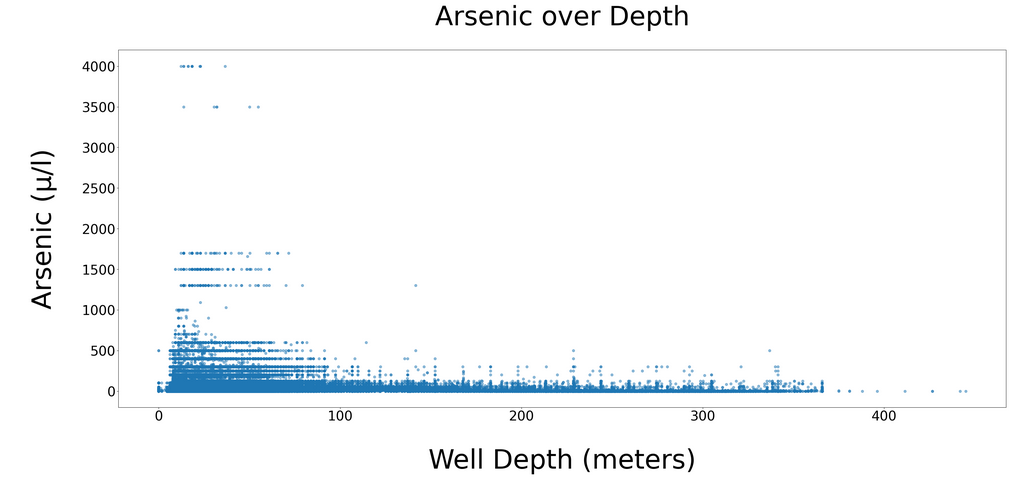
\includegraphics[scale=0.43]{figures/arsenic_over_depth.png} 
    \caption{Distribution of Well Data by District in iArsenic Processed Dataset}
    \label{fig:x aod}
\end{figure}

\textbf{Data Preprocessing \& Feature Engineering}

Model13 trains a separate model for each depth strata. This eliminates the possibility of all nearest neighbours of a data point being from the same region at a different depth. 

Comparing a neighbouring data point at a different depth is wrong because deeper wells will almost always be safer. Therefore wells in the same depth range should be used as neighbours.

In addition to being split into separate depth categories, all features are removed apart from the latitude and longitude.

\subsection{Model14}

Like model8, model14 splits the data into smaller subsets. Instead of splitting the data by the Division, it is split by the depth category. See \ref{tbl:x m14_config} on page \pageref{tbl:x m14_config} to see the configuration of model14.

\textbf{Data Preprocessing \& Feature Engineering}

The data is reduced to the latitude and longitude of each data point. Every column apart from Depth is dropped. All columns are normalised to between 0 and 1.

\begin{table}
    \centering
    \begin{tabular}{c c c c c} 
         \toprule
         Hidden Layers & Solver & Learning Rate & Epochs & Validation \\ [0.5ex] 
         \midrule
         2 & adam & adaptive & 100 & 20\% of train\\ 
         \bottomrule
    \end{tabular}
    \caption{Model14 MLP configuration}
    \label{tbl:x m14_config}
\end{table}

\section{Conclusion}

This chapter describes the landscape in which the machine learning models have been developed by detailing the practicalities of the available data and the existing iArsenic models.

This illustrates the foundation the machine learning models have been developed upon, explaining their design with regard to the requirements and opportunities presented by the existing work.

In the next chapter, Results and Evaluation, the outcome of the experiment execution is evaluated in the context of the desired outcomes defined in the Methodology in section \ref{desired_outcomes} page \pageref{desired_outcomes}. 
\chapter{Results and Evaluation}

In section \ref{desired_outcomes} on page \pageref{desired_outcomes}, the desired outcomes of the project are described. This chapter critically assesses to what extent these outcomes have been met.

\section{Verifying Bias in Test Train Split}

This section examines the limitations of the evaluation. This is done by measuring the bias in the data, using k-folds cross-validation, shuffle split and hold-out testing.

Note that not all types of bias, such as selection bias, can be measured this way and therefore the impact of these biases remains unknown.

\subsection{Quantifying Bias}

Bias in evaluation is inevitable. In section \ref{sub: data_prep} on page \pageref{sub: data_prep} we specified that the data is shuffled to eliminate ordering bias. However, shuffling the data introduces random bias. 

By using k-folds cross-validation we can generate 5 confusion matrices for each model, one for each k-fold, and then we can measure the standard deviation in the confusion matrix metrics.

Table \ref{tbl:x kf_std_cm} on page \pageref{tbl:x kf_std_cm} shows the mean standard deviation of the true positive and false negative metric between the 5 train test splits is 4.1e-03 and 3.39e-03 respectively. This is equivalent to 0.41\% and 0.39\% standard deviation.

For the purpose of evaluating the models in this project, this deviation between splits is considered insignificant. Therefore evaluations are made on one of the k-fold test train subsets, k1.

\begin{table}
    \centering
    \begin{tabular}{c c c} 
         \toprule
         Model & True Positive $\sigma$ & True Negative $\sigma$ \\
         \midrule
         model3 & 1.75e-03 & 5.36e-04\\
         model4 & 1.78e-03 & 8.51e-04\\ 
         model5 & 1.73e-03 & 1.14e-03\\
         model6 & 4.07e-03 & 3.27e-03\\
         model7 & 2.15e-03 & 4.2e-03\\
         model8 & 1.54e-03 & 3.32e-03\\ 
         model9 & 2.21e-02 & 1.71e-02\\
         model10 & 2.27e-03 & 1.45e-03\\
         model11 & 1.95e-03 & 1.41e-03\\
         model13 & 1.64e-03 & 6.36e-04\\
         model14 & 2.182838e-03 & 6.061164e-04\\
         \hline
         \textbf{mean} & 4.1e-03 & 3.39e-03 \\
         \bottomrule
    \end{tabular}
    \caption{Standard deviation of specificity and sensitivity across each test train split}
    \label{tbl:x kf_std_cm}
\end{table}

\newpage

\section{Desired Outcome 1: Evaluating iArsenic Models}

This section details how desired outcome 1 has been achieved. See the desired outcomes at \ref{desired_outcomes} on page \pageref{desired_outcomes}

Table \ref{tbl:x model_evals} on page \pageref{tbl:x model_evals} shows evaluation metrics of the iArsenic and the machine learning based models, and chart \ref{fig:x mpf1} on page \pageref{fig:x mpf1} shows the f1 scores in this table as a bar chart.

The iArsenic models, model3, model4 and model5, have been developed sequentially with each model improving on the one before. The evaluations show that the models have been improving with each iteration. The evaluation also shows that the best performing iArsenic model, model5, achieved an accuracy of 84\% and an f1 of 82\% and a true negative rate of 85\%. See \ref{fig:x Confusion Matrix mode5 Red Staining} on page \pageref{fig:x Confusion Matrix mode5 Red Staining} for a confusion matrix of model5.

Compared to the other models in the literature review, this appears to be a very high level of performance. Though further analysis is required to confirm this as an evaluation metric common to each of these models must be identified. 

\subsection{Benefit of Evaluation of iArsenic Models}

Evaluating the iArsenic models validates their performance and quantifies their suitability for implementation in the iArsenic web application. This facilitates a more informed application of predictions from these models.

The evaluation shows that the performance of the models is increasing with each iteration from model3 to model5, indicating that performance has not plateaued so the development of further models may produce further improvements in performance.

If new iArsenic models are developed, the evaluation of the existing models will be able to indicate where the existing models are underperforming, aiding the development of new models.

The benefit of this evaluation supports the notion that geoscientists should about learn machine learning and artificial intelligence, as the tools and techniques required to generate this kind of evaluation are core in the field of machine learning. 

\subsection{Desired Outcome Achievement}

Prior to this project, there was no evaluation of the iArsenic models. While each iteration was more sophisticated than the last and was presumed to perform better, this was not verifiable.

Because of the evaluations done in this project, it is now verifiable that the models do perform well.

The confusion matrices produced for each model offer a detailed evaluation of the performance of each model. While other evaluation techniques such as receiver operator curves were considered, not all models were able to generate them.

Confusion matrix metrics are displayed in table \ref{tbl:x model_evals} on page \pageref{tbl:x model_evals}.

\newpage

\section{Desired Outcome 2: Comparing iArsenic to Machine Learning Models}

\cite{Fleming2021} makes the case that because of the prevalence of artificial intelligence in earth and environmental science, earth and environmental science students should be taught machine learning and artificial intelligence skills to give geoscientists the ability to work with machine learning concepts more effectively than they currently do, usually with self taught skills.

This project provides an opportunity for a case study wherein existing expert system models, developed by the geoscientist Dr Mohammed Hoque for iArsenic, are compared with machine learning based models.

This section will analyse the benefits and limitations machine learning has brought to iArsenic throughout the development of this project.

\subsection{iArsenic \& Machine Learning Models Performance}

By f1 score, the best performing iArsenic model, model5, achieves a score of 82\%. The best machine learning model is model6, with an f1 score of 72\%. This demonstrates that machine learning models do not inherently produce better performance than expert system models.

This indicates that the models made by a geoscientist without a background in machine learning outperformed machine learning based models. This could indicate that geoscientists may not benefit from machine learning and artificial intelligence education.

\subsection{Desired Outcome Achievement}

The development and comparison of iArsenic models to machine learning models show that machine learning models are able to produce generalised predictions. This proves that machine learning models are applicable to the iArsenic dataset in a comparable way to the existing models. It is probable that with further work machine learning models, like the ones developed in this project, could outperform the existing models. 

\section{Conclusion}

Evaluating the iArsenic models and comparing them to machine learning based models has been a success.

The evaluation of the iArsenic models is a valuable contribution to the application and development of the iArsenic models and iArsenic more broadly. The tools and techniques required to generate these evaluations are rooted in machine learning and artificial intelligence. It could be argued, specifically in the case of iArsenic, that if these skills were more prevalent in geoscience, this would provide a significant benefit. This reinforces the case made in \cite{Fleming2021}.

This project also shows that machine learning is no silver bullet. While the benefit of evaluation is clear, the best performing models in this project were developed specifically from a geoscience background. Indicating that machine learning is not required by geoscientists to make predictive models. This arguably weakens the case made in \cite{Fleming2021}, though with refinement it is possible that machine learning based models could perform at least as well as the expert models, especially if more sophisticated model frameworks are considered.

To conclude, while machine learning skills are valuable, increasing collaboration between geoscience and computer science may be a more practical route to the same effect as increasing machine learning education in geoscience.

\begin{figure}[h]
    \centering
    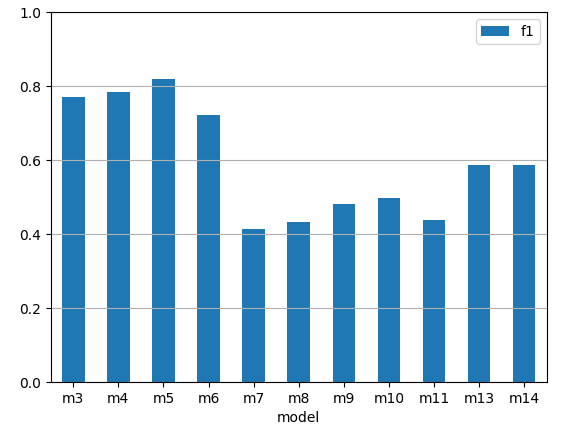
\includegraphics[scale=0.6]{figures/model_f1_barchart.png} 
    \caption{Model performance by f1 score}
    \label{fig:x mpf1}
\end{figure}

\begin{table}
    \centering
    \begin{tabular}{c c c c c c} 
         \toprule
         Model & True Positive & True Negative & f1 & accuracy & precision\\
         \midrule
         model3 & 0.719387 & 0.880010 & 0.771552 & 0.807386 & 0.831874\\
         model4 & 0.741016 & 0.876879 & 0.784060 & 0.815450 & 0.832413\\ 
         model5 & 0.814367 & 0.854302 & 0.818085 & 0.836246 & 0.821837\\
         model6 & 0.725523 & 0.763088 & 0.720984 & 0.746103 & 0.716502\\
         model7 & 0.378534 & 0.623378 & 0.412596 & 0.512674 & 0.453395\\
         model8 & 0.414230 & 0.587080 & 0.432714 & 0.508927 & 0.452924\\
         model9 & 0.410958 & 0.753969 & 0.480913 & 0.598880 & 0.579569\\
         model10 & 0.447443 & 0.706891 & 0.497044 & 0.589187 & 0.559013\\
         model11 & 0.421738 & 0.579780 & 0.437537 & 0.508081 & 0.454565\\
         model13 & 0.663838 & 0.503931 & 0.585893 & 0.576156 & 0.524328\\
         model14 & 0.663940 & 0.503868 & 0.585936 & 0.576167 & 0.524335\\
         \bottomrule
    \end{tabular}
    \caption{Table of evaluation metrics for all models}
    \label{tbl:x model_evals}
\end{table}
\chapter{Limitations \& Future Work}

\section{Limitations}

\textbf{Test Train Split Aggregation}

In some of the models, the test and train data are combined to normalise the data. This is to prevent data points in the test split with features larger than any data point in the test split exceeding a normalized value of 1. 

This is not correct as the train set should be isolated from the model during training.

While this does negatively impact the credibility of the evaluations of the models which have used this technique, the difference made is not likely to be significant enough to change the conclusions or future work in this project.

\textbf{Common Model Interface Removes Index}

The common model interface has been designed to prioritise integration between the NodeJS models and the scikit-learn models. Because both of these model types can read a CSV file, the interface is restricted to passing a CSV file path.

By passing a CSV file path, the DataFrame index is not kept. This blocks model12 from splitting a DataFrame, passing these splits to other models, and then reinserting the predictions into the same row the prediction came from.

Model12 therefore cannot be completed due to a limitation of the common model interface, a solution where the index is maintained would allow models of this type to be explored.

\textbf{Latitude \& Longitude Preprocessing}

Currently, the latitude and longitude preprocessing uses the centroids on the Unions only, not the Mouzas. This is because the function used to merge the geodata to the well data is unable to match the geodata Mouzas and the well data Mouzas, the reason why is not clear. 

With the Mouza centroids, higher resolution latitudes and longitudes could be provided to the models, allowing for more precise decision boundaries to be found.

\textbf{Further Analysis of Neural Network Models}
\label{fannm}

Further analyses of the neural networks will identify what their current limitations are and how they should be further developed to overcome these limitations.

Figure \ref{fig:x lc_m9} on page \pageref{fig:x lc_m9} shows the loss curve of model9 with 2 hidden layers of 50 nodes then 2 nodes. This shows that the decrease in loss is plateauing at 30 iterations, suggesting that further iterations will not provide a significant performance improvement. 

Figure \ref{fig:x lc_big_m9} on page \pageref{fig:x lc_big_m9} shows the sane neural network but with 3 layers of hidden nodes with 2000, 1000 and 100 nodes respectively. After 30 iterations, this model outperforms the model9 instance with less hidden nodes in terms of both performance and training loss. The tradeoff is more computational power being required, causing longer training and test time per iteration. 

The larger model, figure \ref{fig:x lc_big_m9}, is continuing to decrease loss by iteration 30. The larger model does however show signs of overfitting as the difference between the test and the train loss is increasing. This could potentially be mitigated with a larger validation split.  

This shows that more hidden nodes in the neural network produces better performance, though it has not been practical to test these models due to hardware limitations and time constraints.

\begin{figure}[!htb]
    \centering
    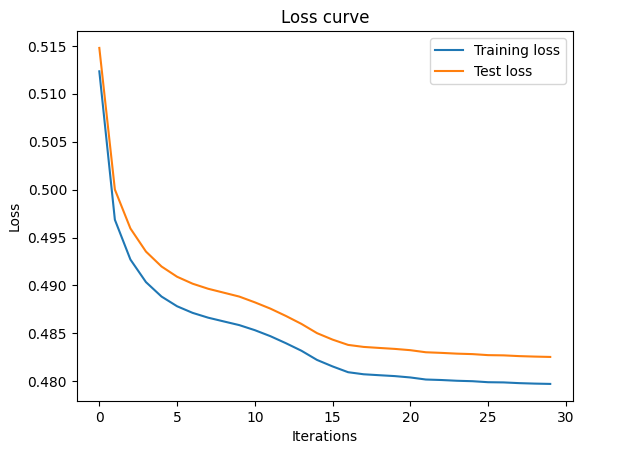
\includegraphics[scale=0.6]{figures/m9_loss_curve.png} 
    \caption{Model9 loss curve 50, 2 hidden layers}
    \label{fig:x lc_m9}
    
    \centering
    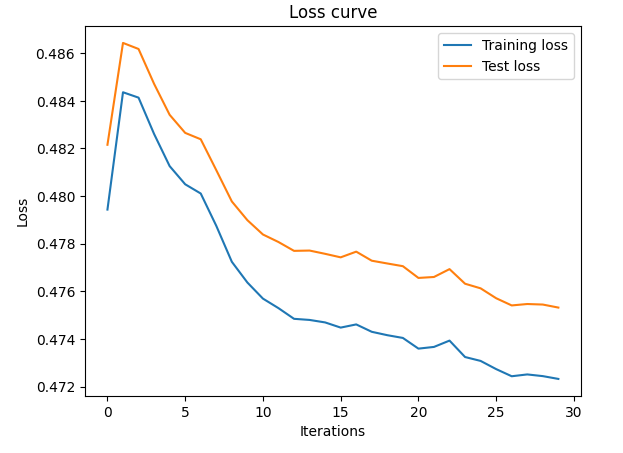
\includegraphics[scale=0.6]{figures/big_nn_loss_curve.png} 
    \caption{Model9 loss curve 2000, 1000, 100 hidden layers}
    \label{fig:x lc_big_m9}
\end{figure}

\section{Future Work}

\subsection{Further Data Integration}

\textbf{Flooding}

\cite{Connolly2022} states that flooding is a "key driver" of groundwater arsenic levels in southeast Asia. Preliminary investigations show that flooding data does exist, but is not readily available in a format which can be integrated into this project without significant preprocessing.

This preprocessing of available flooding data to produce a generic flooding data source could improve the performance of the iArsenic models, potentially achieving new performance records, or form the basis for new machine learning based models.

\textbf{River Geographic Data}

Polygon data for rivers in Bangladesh are readily available for download online. Because flooding tends to happen on riverbanks (see \cite{Connolly2022}), integrating river data into the existing models could be a convenient way to see if further work on higher quality flooding data will be worthwhile.

\textbf{Soil Parameters}

\cite{Winkel2008} shows data from the Food and Agriculture Organization of the United Nations correlates with groundwater arsenic pollution. Integrating this into the available data could allow new models to be trained or existing models to be improved.

\textbf{Elevation}

\cite{Connolly2022} excluded areas with slopes greater than 0.1 degrees from their model because arsenic pollution tends to occur in flat areas. Integrating this data would enable the optimization of the machine learning models, neural network based models in particular, as sloped regions could be ignored by the model.

\subsection{Different Model Types}

\textbf{Convolutional Neural Network Based Model}
\label{cnnbm}

In section \ref{fannm} on page \pageref{fannm} evidence is provided that the model9 neural network with the same design but more hidden nodes and layers perform better. But how many nodes and layers would be ideal?

There is no single rule for how many hidden nodes to use in a neural network, though in mode8, each layer uses half the number of neurons in the previous layer.

Following this rule, for 9,550 Mouzas, each with a latitude and longitude, the perfect network would have 19,100 input nodes (9,550 * 2) and 2 output nodes for a binary classification of 'safe' or 'polluted'. This would result in 12 hidden layers containing a total of 19,090 hidden nodes. This is an impossibly large neural network to implement.

This impossibly large design would allow the entire dataset to fit into the model without optimizing the dataset at the cost of key features.

With a convolutional neural network, these key features could be retained by passing one section of the dataset to the model at a time. The model could then identify patterns to look for within a radius of a data point's latitude and longitude instead of considering it in the context of the entire dataset. This should not impact performance as a data point is likely not dependent on far away data points.

The data is currently split by Division in model8 and depth strata in model14. These manual methods of splitting the data make assumptions about where decision boundaries should be, where a neural network should be able to identify these boundaries with training. Manually splitting the data also reduces the amount of data the model can learn from. Because a convolutional neural network would not require the data to be split into smaller datasets trained on multiple models, these disadvantages could be eliminated.

\textbf{Ensemble Model}

The Evaluation chapter shows that some models perform better than others, what is still not clear, however, is how often the best model outperforms the other models.

The plan for model12 is to take a training set, train and test every other model on the training set, see which model performs best for each region then pass data points in the test set to the model which performs best in that region.

A CSV of the best model for each Upazila can be see here at the following link, this data could not be used by an ensemble model however because this data has been generated from the test set: \url{https://github.com/JavaRip/UoP-SoftEng-Dissertation/blob/main/models/model12/best_model_by_upa.csv}

\textbf{Deep Learning Models \& Pruning}

Investigation of deep learning models has been designated outside the scope of this project. Features introduced by deep learning would allow for new model paradigms to be explored and reduce the negative impact on performance inflicted by current optimization techniques.

Neural network pruning for example could allow neural network models which convert regions to their latitude and longitude to work with higher precision and more detailed region sizes (Mouzas instead of Unions for example). 

Currently, an input node must exist for every point within a square which covers Bangladesh, including areas in neighbouring countries or the ocean. Implementing neural network pruning could allow these regions to be ignored by the model, instead of existing in the model to no benefit. The introduction of flooding, soil and evaluation parameters could also be aided by pruning.

\subsection{Further Development of iArsenic Models}

\textbf{Classification Threshold Manipulation}

The evaluation of the iArsenic models, and the machine learning models which required a common evaluation method, is limited by the inability to generate a receiver operator curve. This is because it is not possible to adjust the classification threshold of the iArsenic models. It would be possible to add this feature by changing the code in the iArsenic models.

\textbf{Future Work Detailed in iArsenic Repository}

The evaluation of the iArsenic models showed that they have increased in performance with each iteration. Further refinements to these models are detailed in the iArsenic repository so it is feasible that further iterations will garner further performance benefits.

\section{Conclusion}

There are four broad categories for future work, developing features to eliminate limitations, developing new models, integrating additional data and continuing development of the iArsenic models.

The most promising area of future development is the development of convolutional neural network models as this continues to expand on the research question, how do machine learning moels compare to the existing iArsenic models, by introducing further machine learning paradigms.
\chapter{Reflection \& Conclusion}

\section{Research Questions}

\subsection{What is the performance of the existing iArsenic models}

Table \ref{tbl:x model_evals} on page \pageref{tbl:x model_evals} shows a thorough analysis of the existing iArsenic models.

These models are deployed in the iArsenic web application and this evaluation provides a key and valuable contribution which was not available before.

This project showed that the performance of the deployed iArsenic model, model5, performs at least as well or better than other models examined in the literature review.

\subsection{Do machine learning models have potential in the prediction of groundwater arsenic pollution?}

While none of the machine learning models outperformed the iArsenic models, model6, model13 and model14 each achieved an f1 score of 58\% or higher.

% TODO reference loss curve in future work
While model6, a random forest classifier and model13, a k-nearest neighbours classifier may be reaching their full potential in this implementation, the feed forward neural network classifiers show potential for further performance improvements with more computing power, optimization or models based on new frameworks. See \ref{fannm} on page \pageref{fannm} and \ref{cnnbm} on page \pageref{cnnbm}.

Despite not outperforming the expert system models, the machine learning models achieved a performance level comparable to the iArsenic models and the other predictive models in the literature review. Therefore the answer to this research question is yes, machine learning models can predict groundwater arsenic pollution, and it is possible that with further work and potentially the use of convolutional neural networks, the performance of the iArsenic models will be exceeded.

\section{New Models Development Strategy}

When developing new models a large portion of time was spent refining the models. While refinement is important and that without refinement the machine learning models would not have performed as well, much of the time spent refining could have been spent exploring different model types.

I was personally driven by a desire to exceed the performance of the existing models, which was at no point a requirement from the client or a requirement to answer the research questions. This has led to fewer model types being explored and potentially viable model types being undiscovered.

If I was to do this project again, I would focus on developing more and a more diverse range of model types.

\section{Achievement of Personal Goals}

The selection of this project for the dissertation was influenced by my own personal motivations. This project provided an amazing opportunity to develop machine learning and artificial intelligence skills and develop experience in the field of improving access to clean drinking water. This has made working on this project an immense privilege.

In some ways, I am left feeling frustrated at the decisions I made throughout the development of this project which resulted in dead ends, wastes of time and moments where I was stuck and unable to make progress for reasons that now seem so obvious to overcome. Ultimately though this frustration stems from the wisdom I now have which I did not have at the start of this project and that represents a huge success.

Having convolutional neural networks next on the roadmap of the development of my skills simply feels unbelievable, as I feel the opportunity to have a working knowledge of cutting edge artificial intelligence and machine learning methodology is now achievable.

Developing this understanding of machine learning and working on a good, worthwhile cause has been immensely personally fulfilling and I am grateful for the opportunities this project has presented.

\section{Conclusion}

This project has been a success, answering the research questions via the desired outcomes and making a genuine contribution to an existing project, iArsenic.

There is more work to do in this project and to the benefit of iArsenic more generally, including some exciting opportunities in deep learning, with this project providing the foundation for this further work.
%\chapter{References}

Bindal, S., \& Singh, C. K. (2019). Predicting groundwater arsenic contamination: Regions at risk in highest populated state of India. Water research, 159, 65-76.\\

Caruana, R., \& Niculescu-Mizil, A. (2006, June). An empirical comparison of supervised learning algorithms. In Proceedings of the 23rd international conference on Machine learning (pp. 161-168).\\

Castelvecchi, D. (2016). Can we open the black box of AI?. Nature News, 538(7623), 20.\\

Connolly, C. T., Stahl, M. O., DeYoung, B. A., \& Bostick, B. C. (2021). Surface flooding as a key driver of groundwater arsenic contamination in Southeast Asia. Environmental Science \& Technology, 56(2), 928-937.\\

Chakraborti, D., Rahman, M. M., Das, B., Murrill, M., Dey, S., Mukherjee, S. C., ... \& Quamruzzaman, Q. (2010). Status of groundwater arsenic contamination in Bangladesh: a 14-year study report. Water research, 44(19), 5789-5802.\\

Connolly, C. T., Stahl, M. O., DeYoung, B. A., \& Bostick, B. C. (2021). Surface flooding as a key driver of groundwater arsenic contamination in Southeast Asia. Environmental Science \& Technology, 56(2), 928-937.\\

Fleming, S. W., Watson, J. R., Ellenson, A., Cannon, A. J., \& Vesselinov, V. C. (2021). Machine learning in Earth and environmental science requires education and research policy reforms. Nature Geoscience, 14(12), 878-880.\\

Géron, A. (2017). Hands-on machine learning with scikit-learn and tensorflow: Concepts. Tools, and Techniques to build intelligent systems.\\

Ghosh, G. C., Khan, M., Hassan, J., Chakraborty, T. K., Zaman, S., Kabir, A. H. M., \& Tanaka, H. (2020). Human health risk assessment of elevated and variable iron and manganese intake with arsenic-safe groundwater in Jashore, Bangladesh. Scientific reports, 10(1), 1-9.\\

Guidotti, R., Monreale, A., Ruggieri, S., Turini, F., Giannotti, F., \& Pedreschi, D. (2018). A survey of methods for explaining black box models. ACM computing surveys (CSUR), 51(5), 1-42.\\

Khan, N. I., \& Yang, H. (2014). Arsenic mitigation in Bangladesh: An analysis of institutional stakeholders' opinions. Science of the total environment, 488, 493-504.\\

Loyola-Gonzalez, O. (2019). Black-box vs. white-box: Understanding their advantages and weaknesses from a practical point of view. IEEE Access, 7, 154096-154113.\\

Najafabadi, M. M., Villanustre, F., Khoshgoftaar, T. M., Seliya, N., Wald, R., \& Muharemagic, E. (2015). Deep learning applications and challenges in big data analytics. Journal of big data, 2(1), 1-21.\\

Smith, A. H., Lingas, E. O., \& Rahman, M. (2000). Contamination of drinking-water by arsenic in Bangladesh: a public health emergency. Bulletin of the World Health Organization, 78(9), 1093-1103.\\

Van Halem, D., Bakker, S. A., Amy, G. L., \& Van Dijk, J. C. (2009). Arsenic in drinking water: a worldwide water quality concern for water supply companies. Drinking Water Engineering and Science, 2(1), 29-34.\\

Winkel, L., Berg, M., Amini, M., Hug, S. J., \& Annette Johnson, C. (2008). Predicting groundwater arsenic contamination in Southeast Asia from surface parameters. Nature Geoscience, 1(8), 536-542.\\

World Health Organization. (2003). Arsenic in drinking-water: background document for development of WHO guidelines for drinking-water quality (No. WHO/SDE/WSH/03.04/75). World Health Organization.\\

%%%%%%%%%%%%%% REFERENCES SECTION
\newpage
\phantomsection
\addcontentsline{toc}{chapter}{References}
% In order to try and get a consistent format I copy and paste the INSPIRE bibtex code into my bibtex file.
\printbibliography

%%%%%%%%%%%% Include your appendices here

\appendix

\chapter{Appendix}

\section{Colorblind Compatible Figures}

\begin{figure}[!htb]
    \centering
    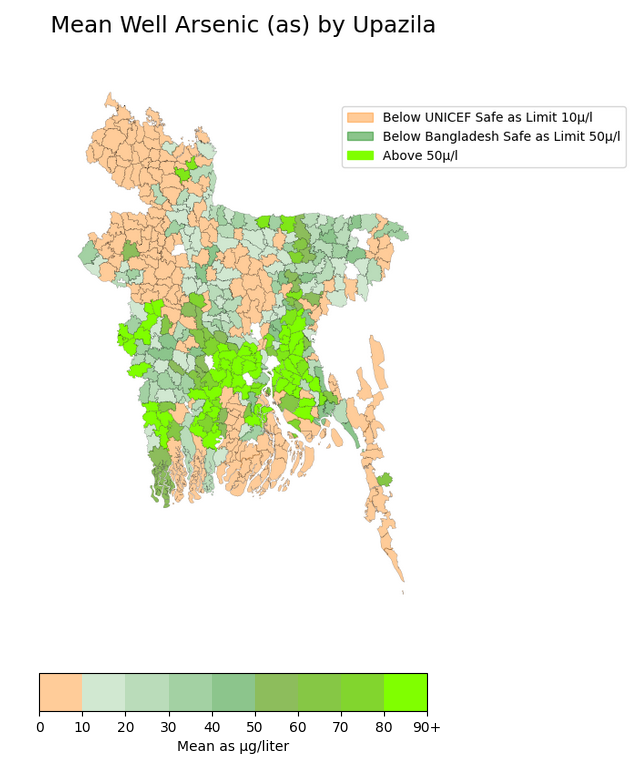
\includegraphics[scale=0.6]{appendix/cblind_as_by_upa.png} 
    \caption{Red excluded for red / green colourblind: Distribution of Average (mean) Arsenic by Upazila in the iArsenic Standard Dataset}
    \label{fig:x avg_as_cblind}
\end{figure}

\section{PID}


\includepdf[pages={1-},scale=1]{appendix/PID.pdf}

\end{document}
